\documentclass[a4paper,12pt]{article}[abntex2]
\bibliographystyle{abntex2-alf}
\usepackage{siunitx} % Fornece suporte para a tipografia de unidades do Sistema Internacional e formatação de números
\usepackage{booktabs} % Melhora a qualidade das tabelas
\usepackage{tabularx} % Permite tabelas com larguras de colunas ajustáveis
\usepackage{graphicx} % Suporte para inclusão de imagens
\usepackage{newtxtext} % Substitui a fonte padrão pela Times Roman
\usepackage{ragged2e} % Justificação de texto melhorada
\usepackage{setspace} % Controle do espaçamento entre linhas
\usepackage[a4paper, left=3.0cm, top=3.0cm, bottom=2.0cm, right=2.0cm]{geometry} % Personalização das margens do documento
\usepackage{lipsum} % Geração de texto dummy 'Lorem Ipsum'
\usepackage{fancyhdr} % Customização de cabeçalhos e rodapés
\usepackage{titlesec} % Personalização dos títulos de seções
\usepackage[portuguese]{babel} % Adaptação para o português (nomes e hifenização
\usepackage{hyperref} % Suporte a hiperlinks
\usepackage{indentfirst} % Indentação do primeiro parágrafo das seções
\sisetup{
  output-decimal-marker = {,},
  inter-unit-product = \ensuremath{{}\cdot{}},
  per-mode = symbol
}
\setlength{\headheight}{14.49998pt}

\DeclareSIUnit{\real}{R\$}
\newcommand{\real}[1]{R\$#1}
\usepackage{float} % Melhor controle sobre o posicionamento de figuras e tabelas
\usepackage{footnotehyper} % Notas de rodapé clicáveis em combinação com hyperref
\hypersetup{
    colorlinks=true,
    linkcolor=black,
    filecolor=magenta,      
    urlcolor=cyan,
    citecolor=black,        
    pdfborder={0 0 0},
}
\usepackage[normalem]{ulem} % Permite o uso de diferentes tipos de sublinhados sem alterar o \emph{}
\makeatletter
\def\@pdfborder{0 0 0} % Remove a borda dos links
\def\@pdfborderstyle{/S/U/W 1} % Estilo da borda dos links
\makeatother
\onehalfspacing

\begin{document}

\begin{titlepage}
    \centering
    \vspace*{1cm}
    \Large\textbf{INSPER – INSTITUTO DE ENSINO E PESQUISA}\\
    \Large ECONOMIA\\
    \vspace{1.5cm}
    \Large\textbf{Slides - H.E.B}\\
    \vspace{1.5cm}
    Prof. Heleno Piazenini Vieira\\
    Prof. Auxiliar \\
    \vfill
    \normalsize
    Hicham Munir Tayfour, \href{mailto:hichamt@al.insper.edu.br}{hichamt@al.insper.edu.br}\\
    5º Período - Economia A\\
    \vfill
    São Paulo\\
    Agosto/2024
\end{titlepage}

\newpage
\tableofcontents
\thispagestyle{empty} % This command removes the page number from the table of contents page

\newpage 
\listoffigures
\thispagestyle{empty} % This command removes the page number from the table of contents page

\newpage
\setcounter{page}{1} % This command sets the page number to start from this page
\justify
\onehalfspacing

\pagestyle{fancy}
\fancyhf{}
\rhead{\thepage}

\section{\textbf{Aula 2 - Organização econômica colonial}}

\subsection{\textbf{Introdução}}

\begin{itemize}
    \item \textbf{O contexto econômico}
    \begin{itemize}
        \item Primeira onda de expansão comercial dos europeus, lógica do Mercantilismo
    \end{itemize}
    
    \item \textbf{Porque há interesse em povoar o território?}
    \begin{itemize}
        \item Possibilidade de explorar metais preciosos
        \item Povoar é um meio de defesa (há ameaça externa)
    \end{itemize}
    
    \item \textbf{Como a ocupação foi economicamente viabilizada?}
    \begin{itemize}
        \item A partir do sucesso da produção agrícola
        \item Quais razões explicam esse sucesso?
    \end{itemize}
    
    \item \textbf{O que é importante nesta aula?}
    \begin{itemize}
        \item Explicar o sucesso agrícola inicial
        \item Entender por que a mão de obra escrava africana foi a principal
        \item A queda dos preços do açúcar na 2ª metade do XVII provocou o término do ciclo deste produto?
    \end{itemize}
\end{itemize}

\subsection{\textbf{Agricultura: fatores de êxito}}
\begin{itemize}
    \item Experiência portuguesa com o açúcar (ilhas do Atlântico) \begin{itemize}
        \item resolver questões técnicas
        \item fomentou desenvolvimento da “indústria” de equipamentos (engenhos)
        \item mão de obra
    \end{itemize}
    \item Experiência e conhecimento sobre o mercado escravo africano de mão de obra
    \item Contou com a participação holandesa \begin{itemize}
        \item especializados no comércio intra-europeu e grandes financiadores (criar mercado para o açúcar)
        \item financiamento: comércio, refino, instalações e mão de obra
    \end{itemize}
    \item “Razão do monopólio” (fator macroeconômico)
\end{itemize}

\subsection{\textbf{Agricultura: mão de obra}}
\begin{itemize}
    \item No início: utilização da mão de obra indígena \begin{itemize}
        \item a operação agrícola ainda não está consolidada (demanda reduzida por escravos)
        \item população portuguesa não demonstra interesse dada a importância do Oriente
    \end{itemize}
    \item Porque os escravos nativos não persistem como mão de obra principal? \begin{itemize}
        \item Freyre, Furtado e Prado Jr explicam, mas...
        \item interesse dos traficantes que operam o comércio negreiro;
        \item questão biológica (Alfred Crosby);
        \item correntes e ventos do Atlântico Sul e o problema da interligação territorial brasileira (L. F. Alencastro).
    \end{itemize}
\end{itemize}

\begin{figure}[H]
    \centering
    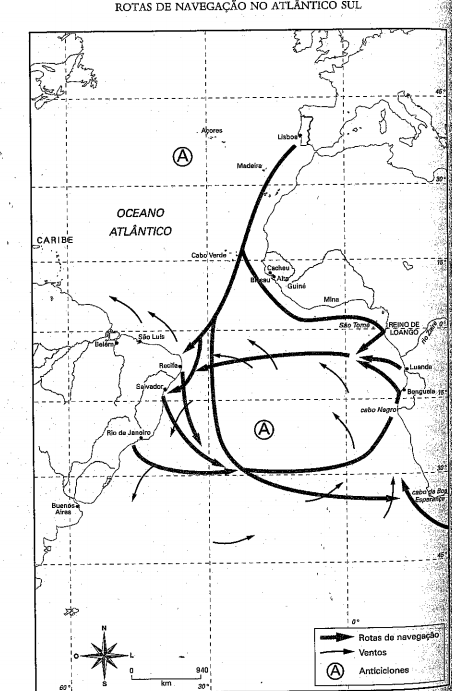
\includegraphics[width=0.5\textwidth]{Imagens Slides/i1a2.png}
    \caption{Correntes e Ventos do Atlântico Sul}
\end{figure}

\subsection{\textbf{Narrativa diante de evidências}}

\begin{itemize}
    \item Na 2ª metade do século XVII temos forte queda dos preços do açúcar com a entrada de mais produtores (Antilhas) \begin{itemize}
        \item o Nordeste açucareiro entra em crise;
        \item o ciclo do açúcar termina e começa o ciclo do ouro; (o que isso quer dizer?)
    \end{itemize}
    \item Estagnação econômica do Nordeste (Furtado). Isso, de fato aconteceu? O que as evidências mostram?
\end{itemize}

\begin{figure}[H]
    \centering
    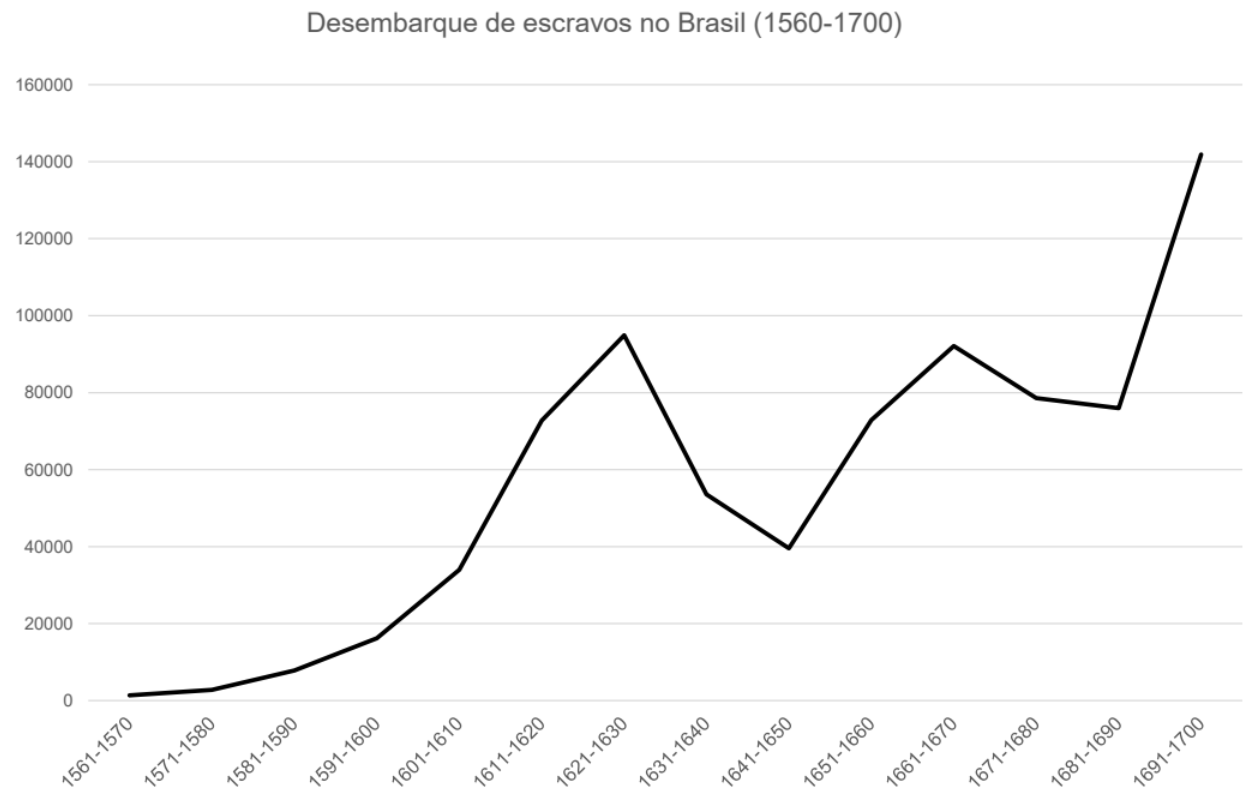
\includegraphics[width=0.7\textwidth]{Imagens Slides/i2a2.png}
    \caption{Desembarque de escravos no Brasil (1560-1700)}
\end{figure}

\begin{figure}[H]
    \centering
    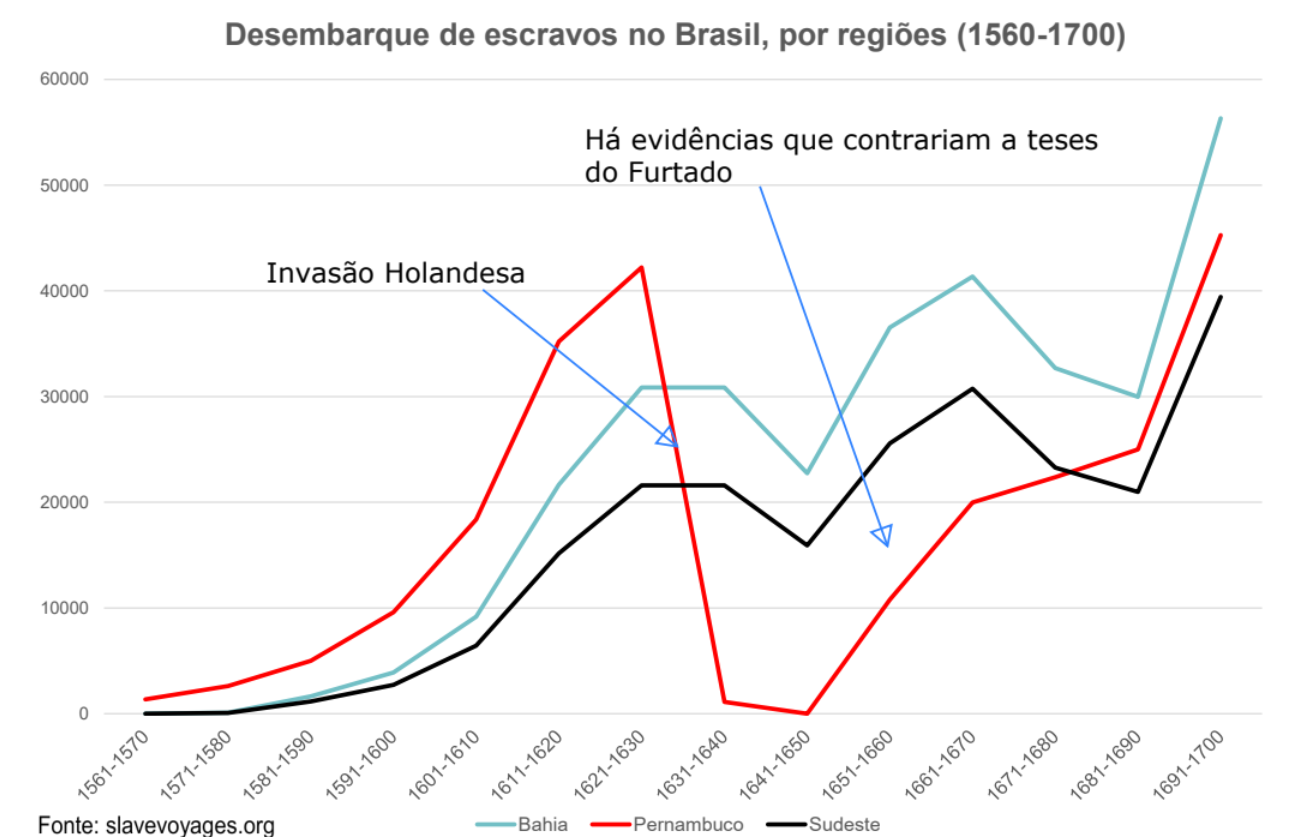
\includegraphics[width=0.7\textwidth]{Imagens Slides/i3a2.png}
    \caption{Desembarque de escravos no Brasil, por regiões (1560-1700)}
\end{figure}

\subsection{\textbf{Conclusão}}
\begin{itemize}
    \item O que aprendemos nessa aula? \begin{itemize}
        \item notar a participação holandesa para explicar o sucesso da economia açucareira no século XVI/XVII; 
        \item aplicar teoria macro para explicar o sucesso da economia açucareira no século XVI/XVII;
        \item refletir sobre a lógica econômica do uso de escravos africanos;
        \item considerar evidências: sugerem que o aumento da concorrência no mercado do açúcar e a queda de seu preço não trouxeram regressão econômica do Nordeste no final do século XVII.
    \end{itemize}
\end{itemize}
\newpage

\section{\textbf{Aula 3 - Organização econômica colonial (parte 2)}}

\subsection{\textbf{Introdução}}
"O ouro brasileiro deixou igrejas em Portugal, fábricas na Inglaterra e buracos no Brasil”
O que é importante?
\begin{itemize}
    \item Resposta: Estabelecer uma visão crítica sobre a dinâmica econômica da mineração a partir da interpretação de Celso Furtado. 
    \item Descoberta do Ouro (final do século XVII - 1690)
    \begin{itemize}
        \item novo impulso para o crescimento econômico colonial;
        \item a extração é contínua de 1690 até 1760;
        \item informação da descoberta rapidamente transmitida: forte migração interna e externa;
        \item houve surgimento de centros urbanos (ofertar serviços para extração). 
    \end{itemize}
\end{itemize}

\subsection{\textbf{Temas importantes em Minas}}
\begin{enumerate}
    \item O mercado interno
    \begin{enumerate}
        \item O que Furtado diz sobre o mercado interno?
        \begin{enumerate}
            \item Resposta: O meio socioeconômico é mais complexo
        \end{enumerate}
    \end{enumerate}
    \item O tamanho da concentração (desigualdade)
    \item O termo "Decadência)
\end{enumerate}
\subsection{\textbf{Furtado: Açúcar X Minas}}
\begin{itemize}
    \item Meio social mais complexo \begin{itemize}
        \item escravos não são maioria
        \item mobilidade social maior
    \end{itemize}
    \item Estrutura de custo fixo menor
    \item Especialização requer atividades acessórias \begin{itemize}
        \item dificuldades no abastecimento (fome e $\uparrow{preços}$)
        \item preços maiores estimulam atividades acessórias
        \item menor grau de importações
    \end{itemize}
    \item Sistema de transportes \begin{itemize}
        \item localização geográfica e solo ruim
        \item grande demanda por animais de carga
    \end{itemize}
\end{itemize}

\begin{figure}[H]
    \centering
    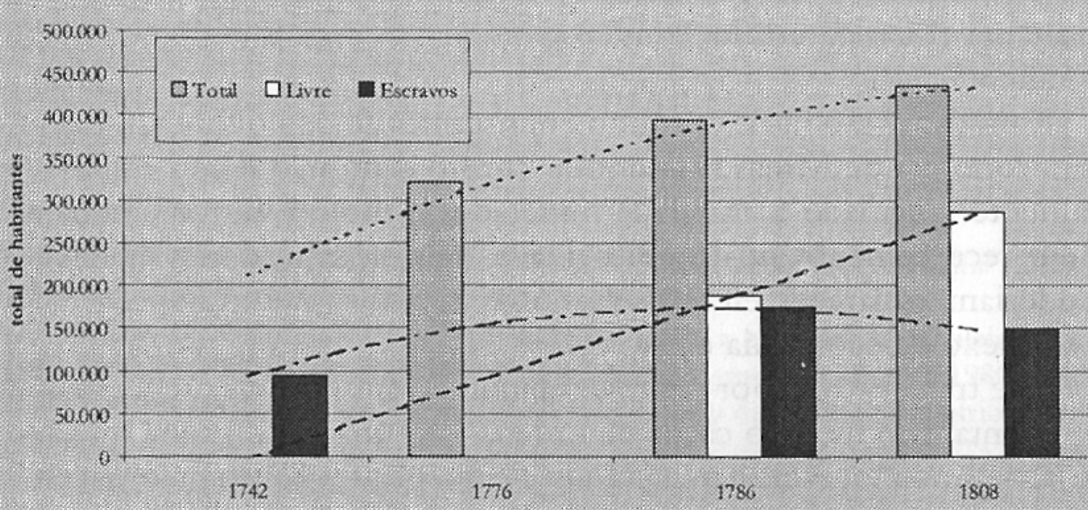
\includegraphics[width=0.7\textwidth]{Imagens Slides/i1a3.png}
    \caption{Evidências – População total da Capitania de Minas Gerais (1742-1808)}
\end{figure}

\subsection{\textbf{Discussão sobre o potencial do mercado interno mineiro}}
\begin{itemize}
    \item Como podemos diferenciar o potencial de mercado interno nordestino do mineiro? \begin{itemize}
        \item o que mudou na Colônia?
        \item fatores de produção da Colônia pouco desenvolvidos (integração reduzida com o setor manufatureiro)
        \item porque a atividade manufatureira não se desenvolve na Colônia?
    \end{itemize}
    \item Como podemos conectar essa discussão com o Tratado de Methuen (1703) e com o contexto global do séc. XVIII?
\end{itemize}

\subsection{\textbf{Possível conectar Minas com o “mundo”?}}
\begin{itemize}
    \item Revolução Industrial \begin{itemize}
        \item Institucionalistas (North), fatores internos importam! 
        \item \textbf{VS}
        \item Marxistas (“Furtado”, Prado Jr, Novais), fatores externos importam!
    \end{itemize}
    \item Como sair dessa dicotomia? \begin{itemize}
        \item Novamente os institucionalistas
    \end{itemize}
\end{itemize}

\subsection{\textbf{Comércio no Atlântico Sul importa!}}

Testam a importância dos lucros obtidos no comércio do Atlântico Sul para explicar desenvolvimento econômico  europeu

O comércio e as atividades coloniais afetam diretamente a Europa e também indiretamente, induzindo à transformações institucionais

Crescimento comercial no Atlântico Sul permitiu que comerciantes enfrentassem a monarquia centralizada, obtiveram instituições para proteger direitos de propriedade

Tais mudanças foram centrais para explicar o crescimento econômico no período histórico subsequente.

\subsection{\textbf{Concentração em Minas}}
\begin{itemize}
    \item  O que diz Furtado?
    \item  Uma visão mais crítica \begin{itemize}
        \item evidências, nova pesquisa e de novo E\&S
    \end{itemize}
\end{itemize}

\subsection{\textbf{Efeito econômico do Ouro}}

\begin{itemize}
    \item Não é somente um recurso natural!
    \item Não é uma mercadoria!
    \item É “descoberta” de moeda! \begin{itemize}
        \item portanto, há efeito monetário
        \item que é multiplicador de atividades e de renda
        \item reduz o peso do mercado internacional na explicação das flutuações econômicas internas
        \item mas isso reduziu a concentração econômica colonial?
    \end{itemize}
\end{itemize}

\subsection{\textbf{Como era a concentração de renda em Minas? (Carrara)}}

\begin{itemize}
    \item Concentração de renda é elevada! \begin{itemize}
        \item em 1710, por exemplo, apenas cinco pessoas foram responsáveis por cerca de 47\% de todo o ouro produzido na Intendência do Rio das Mortes.
        \item um século depois, os cinco maiores produtores conseguiram quase 82 quilos de ouro –16 quilos média –, e os 568 menores ficaram com menos de 184 quilos – média de 347 gramas para cada um.
    \end{itemize}
    \item Uma ideia do poder de compra de um quilo de ouro: \begin{itemize}
        \item suficiente para comprar 75 cabeças de gado ou 
2.250 sacos de milho com cerca de 30 quilos cada um.
    \end{itemize}
    \item Assim, uma enorme quantidade de moeda, distribuída por um número de pessoas bem maior, explica o impacto que a mineração tinha sobre a economia local. 
    \item O ouro estimulou a produção de gêneros de muitos setores da economia, especialmente a agricultura e a pecuária voltadas para o abastecimento interno. \begin{itemize}
        \item  poucas pessoas envolvidas na mineração (maior parte da população da capitania morava nos campos e vivia dos trabalhos agrícolas e pastoris). 
        \item extração de ouro, setor que gerava os mais valiosos rendimentos fiscais para a Coroa, mobilizava, no máximo, 5\% dos moradores de Minas Gerais.
    \end{itemize}
\end{itemize}

Conclusão: mesmo com uma concentração de renda elevada foi possível ampliar e diversificar o mercado interno colonial

\subsection{\textbf{Houve ruptura da herança?}}
\begin{itemize}
    \item Retomando o esquema de análise de 
E\&S;
    \item Efeitos de um choque migratório? Como podemos responder esta pergunta diante da discussão anterior? \begin{itemize}
        \item O “modelo” de E\&S se altera?
    \end{itemize}
\end{itemize}


\subsection{\textbf{Decadência em Minas}}
\begin{itemize}
    \item O que diz Furtado?
    \item Uma visão mais crítica \begin{itemize}
        \item evidências, nova pesquisa
    \end{itemize}
    \item Dado o esgotamento das jazidas: \begin{itemize}
        \item Economia mineira “regrediu” para um atividade de subsistência, deixando escravos ociosos e que seriam a base inicial para o surgimento cafeeiro (Furtado)
        \item A “decadência” deve ser lida como uma queda do nível do comércio interno da Capitania decorrente da menor disponibilidade de moeda, isto é, de ouro em pó (Carrara)
    \end{itemize}
\end{itemize}

\begin{figure}[H]
    \centering
    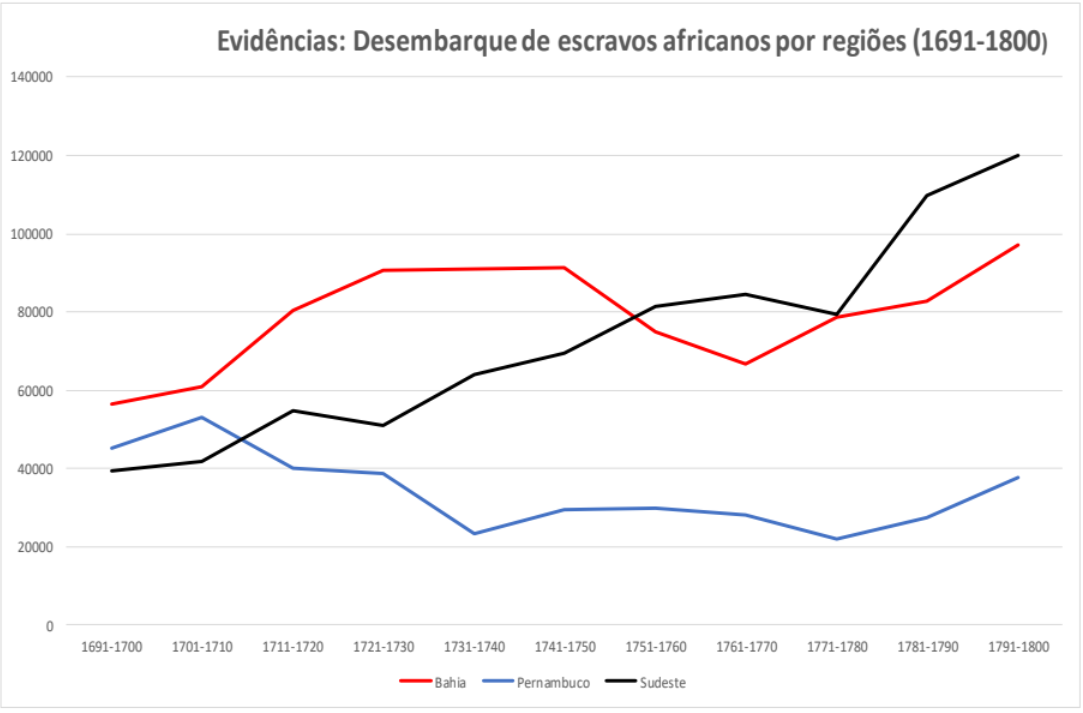
\includegraphics[width=0.7\textwidth]{Imagens Slides/i2a3.png}
    \caption{Evidências: Desembarque de escravos africanos por regiões (1691-1800)}
\end{figure}

Voltando a frase:\textbf{ “O ouro brasileiro deixou igrejas em Portugal, fábricas na Inglaterra e buracos no Brasil”}

\subsection{\textbf{O que aprendemos?}}
\begin{itemize}
    \item Refletir sobre o impacto econômico da descoberta do Ouro.
    \item Identificar e explicar a questão da concentração econômica no contexto do século XVIII
    \item Explicar a dificuldade do surgimento do setor manufatureiro na Colônia no final do século XVIII.
    \item  Pensar e explicar a participação da mineração brasileira no contexto mundial do século XVIII. \begin{itemize}
        \item Como as correntes de pensamento da história econômica explicam a relação entre “Minas” e a Revolução industrial?
    \end{itemize}
    \item Refletir sobre a “decadência” da economia mineira. \begin{itemize}
        \item o que as evidências mostram?
    \end{itemize}
\end{itemize}
\newpage



\section{\textbf{Aula 4 - Discussões sobre a visão tradicional da Colônia}}
\begin{figure}[H]
    \centering
    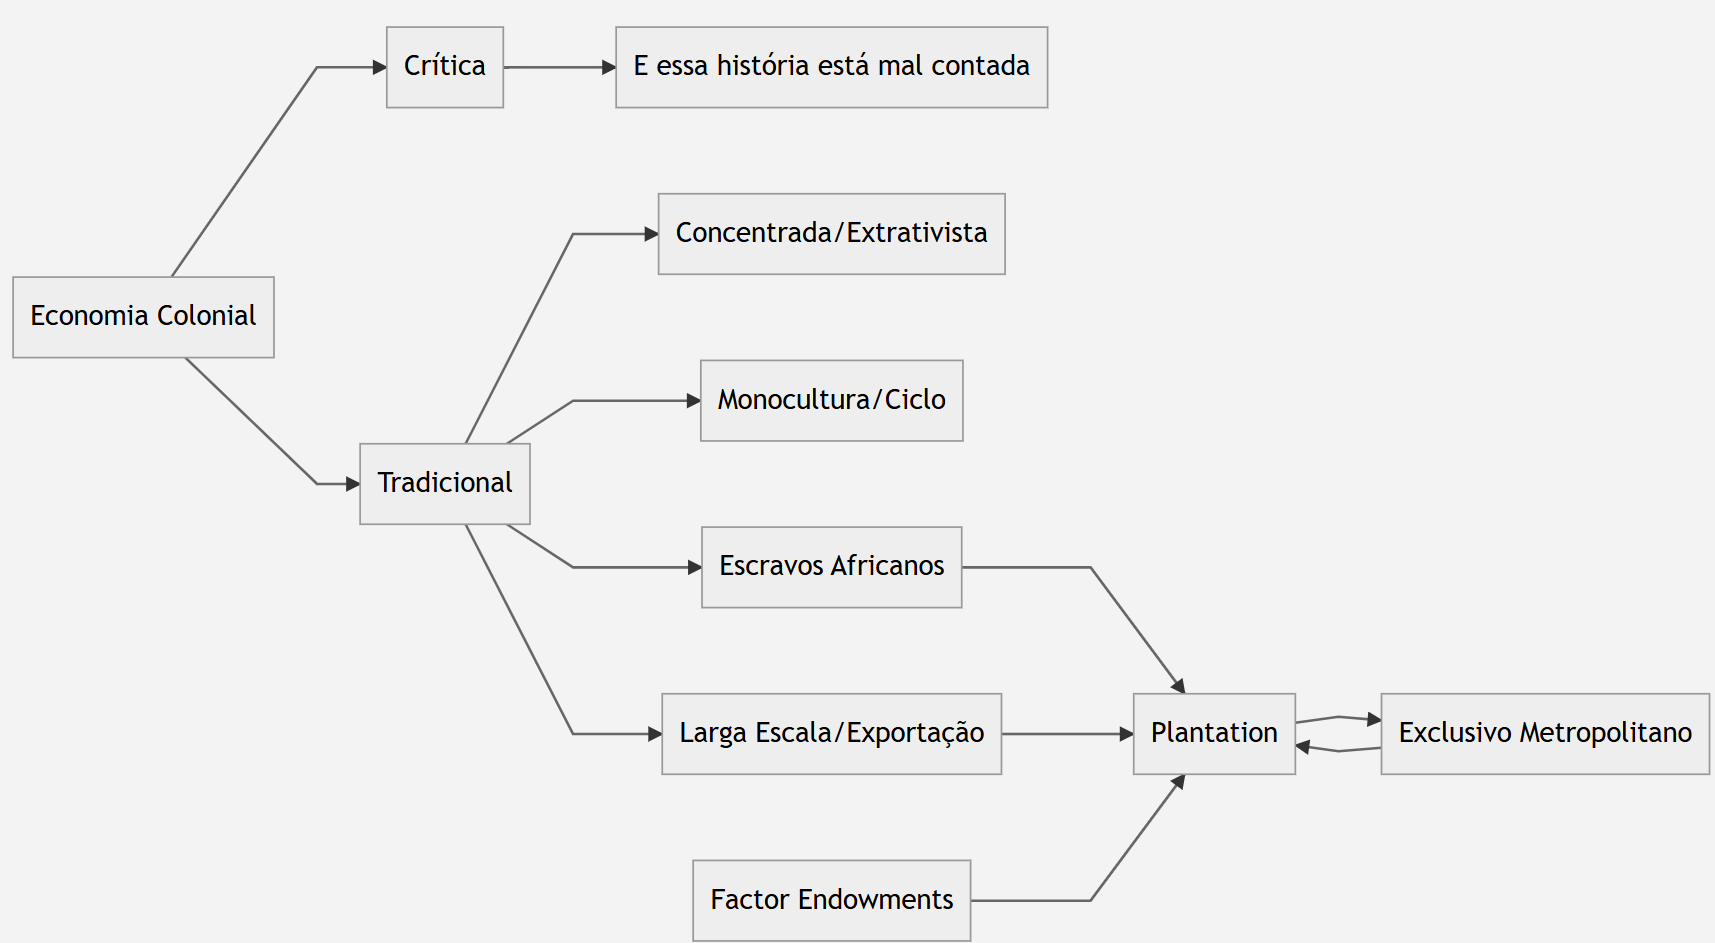
\includegraphics[width=1.0\textwidth]{Imagens Slides/i1a4.png}
\end{figure}

\subsection{\textbf{Introdução}}

\begin{itemize}
    \item Diante do que já estudamos sobre a dinâmica colonial:
    \begin{itemize}
        \item Qual é o papel da Colônia e como foi a formação econômica do Brasil?
        \item Qual foi a estrutura econômica colonial montada?
    \end{itemize}
\end{itemize}

\textbf{O que é importante?}
\begin{itemize}
    \item Responder essas perguntas criticamente, complementando o que já discutimos
    \item Buscar evidências para apoiar a reflexão;
    \item Considerar agenda mais recente de pesquisa.
\end{itemize}


\subsection{\textbf{Organização colonial: como aprendemos?}}

\begin{itemize}
    \item Portugal impõe o exclusivo comercial (ou pela geografia econômica), temos:
    \begin{itemize}
        \item setor de exportação do açúcar predomina (monocultura);
        \item grandes proprietários de terras e de escravos;
        \item mercado interno e outros setores praticamente inexistentes;
        \item colônia totalmente complementar e dependente da Metrópole.
    \end{itemize}
\end{itemize}

\begin{itemize}
    \item Estrutura baseada na mão de obra escrava Africana
    \begin{itemize}
        \item interesse dos comerciantes portugueses;
        \item contato dos portugueses com Africanos;
        \item dificultar o tráfico interno de nativos, evitando concorrência com Africanos.
    \end{itemize}
\end{itemize}


\subsection{\textbf{Síntese}}

\begin{itemize}
    \item Para entender a formação econômica do Brasil estudamos uma região que:
    \begin{itemize}
        \item exporta um único produto e exclusivamente para Portugal;
        \item o ciclo do açúcar termina e na sequência há o ciclo do ouro (ideia de “ciclos” sucessivos baseados em único produto de exportação);
        \item setor exportador é o principal e o mercado interno é \textit{“reduzidíssimo”} (Novais).
    \end{itemize}
\end{itemize}

\begin{itemize}
    \item empresários são grandes proprietários de terras e possuem muitos escravos;
    \item havia uma relação triangular no comércio de escravos (PORT-BRA-ÁFRICA).
\end{itemize}

\begin{itemize}
    \item Em suma: não existe autonomia da Colônia em relação à Metrópole.
\end{itemize}

\subsection{\textbf{Mas...}}

\begin{itemize}
    \item \textit{O Conselho Ultramarino} (1642)
    \begin{itemize}
        \item É uma organização portuguesa que elaborou e executou a política colonial.
        \item A pesquisa em documentos deste conselho mostra que este:
        \begin{itemize}
            \item exigia plantio de cereais, milho, mandioca e feijão;
            \item incentivava vinda de colonos pobres para empreender nas atividades de oferta interna para manter a colônia (por exemplo, evitar a fome);
            \item incentivava geração de excedentes dessa oferta para abastecer outras colônias (e até exportar para a metrópole).
        \end{itemize}
    \end{itemize}
    \item Havia uma produção significativa de tabaco, mandioca e cachaça para exportação que indica uma relação bilateral Brasil-África.
    \item Ou seja, há diversas atividades que produzem:
    \begin{itemize}
        \item vários gêneros para exportação;
        \item exportações são destinadas também para outras colônias (além de Portugal);
        \item para abastecer o mercado interno;
    \end{itemize}
    \item O Brasil importa escravos da África e artigos da Índia.
\end{itemize}

\subsection{\textbf{Agricultura para consumo doméstico e exportação}}

\begin{itemize}
    \item São Paulo se desenvolve como provedor de bens agrícolas:
    \begin{itemize}
        \item atender ao restante da Colônia e exportar para Angola;
        \item Outras atividades - farinha de mandioca, milho, trigo, feijão, carnes, tecidos rústicos...
    \end{itemize}
    \item Três produtos e regiões produtoras com muita importância para o tráfico negreiro:
    \begin{itemize}
        \item Bahia produz tabaco;
        \item RJ produz mandioca e depois cachaça.
    \end{itemize}
\end{itemize}

\begin{figure}[H]
    \centering
    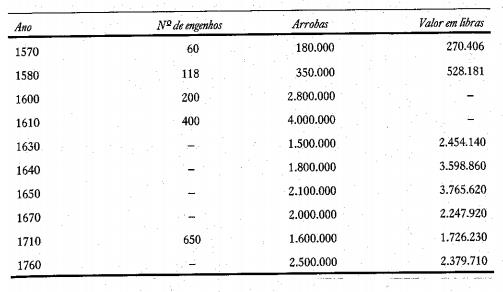
\includegraphics[width=0.7\textwidth]{Imagens Slides/i2a4.png}
    \caption{Evidências: setor açucareiro ao longo do tempo}
\end{figure}

\subsection{\textbf{Algumas conclusões}}

\begin{itemize}
    \item Evidências (dados e documentação) indicam que:
    \begin{itemize}
        \item Colônia possuía pauta diversificada de produção
        \begin{itemize}
            \item exportava vários produtos (não é monocultura);
            \item havia diversas atividades que abasteciam o mercado interno (mercado interno não parece “reduzidíssimo”);
        \end{itemize}
        \item Estrutura econômica era muito mais complexa
        \begin{itemize}
            \item também há pequenos produtores (com poucos escravos cada);
            \item várias regiões têm relevância em momentos históricos concomitantes (não vale a ideia de ciclos econômicos com base em produtos únicos);
        \end{itemize}
    \end{itemize}
\end{itemize}

\subsection{\textbf{Tráfico de escravos africanos}}

\begin{itemize}
    \item Visão tradicional: comércio triangular
    \item No entanto: perto de 85\% dos navios que entravam em Luanda no século XVIII eram brasileiros (principalmente de RJ, PE e BA). Apenas 15\% eram portugueses. \textit{Alencastro (2000)}
    \begin{itemize}
        \item os “brasilícos” eram mais adaptados ao clima e às doenças da África;
        \item Africanos preferem os produtos brasileiros;
        \item as rotas de navegação favoreciam o comércio bilateral África-Brasil (“ventos do comércio negreiro”).
    \end{itemize}
    \item \textbf{Conclusão}: o comércio negreiro era uma atividade liderada por traficantes brasileiros! \textit{Alencastro (2000)}
\end{itemize}

\subsection{\textbf{Objetivos da aula}}
\begin{itemize}
    \item Formar uma visão mais ampla e crítica de como era a organização econômica colonial
    \begin{itemize}
        \item dizer que a Colônia era organizada em grandes propriedades e exclusivamente para exportar açúcar (e depois ouro), talvez seja uma explicação pobre;
        \item o tamanho do mercado interno colonial foi subestimado;
        \item a importância do comércio de escravos para a formação econômica do Brasil é subestimada;
    \end{itemize}
    \item Refletir sobre o sentido da colonização: ele é mais complexo, há mais diversidade (há evidências!)
\end{itemize}

\begin{itemize}
    \item Considerar o raciocínio da Formação do Brasil no Atlântico Sul
    \begin{itemize}
        \item As atividades de mercado interno, as culturas de exportação e o tráfico de escravos devem ser conectados;
        \item Agente econômico importante: traficante de escravos (movimenta a economia colonial, concentra renda etc);
        \item Essa dinâmica impacta nossa formação econômica.
    \end{itemize}
    \item Herança colonial tem de ser mapeada com cuidado! (Exemplo: como E\&S mapearam?)
\end{itemize}
\newpage

\section{\textbf{Aula 5 - Antecedentes da Independência do Brasil 200 anos}}

\subsection{\textbf{Temas e objetivos de aprendizagem}}
\begin{itemize}
    \item O que é importante?
    \begin{itemize}
        \item Refletir sobre as razões da Independência do Brasil (as ideias e os
problemas econômicos envolvidos)
\item Refletir, em termos gerais, sobre os anos 1820
    \end{itemize}
\end{itemize}
\subsection{\textbf{Introdução}}
\begin{itemize}
    \item A importância da análise das escolhas fiscais
    \begin{itemize}
        \item Decisões fiscais indicam os atores importantes e o peso de suas
forças políticas em uma sociedade;
\item  Sinalizam “vencedores e perdedores” na sociedade;
\item Caracteriza o contexto político e sua dinâmica em cada momento
histórico;
\item Em sociedades democráticas liberais, “todos” os grupos sociais
são representados no Parlamento e disputam o orçamento;
\item Por outro lado, em tempos de absolutismo, por exemplo, o
orçamento “é o Rei”

    \end{itemize}
    \item Contexto histórico global e ideias – relação entre Sociedade e Estado
    \begin{itemize}
        \item Período do século XVIII; “A era das revoluções”;
        \item Revolução do Porto e a Queda do Absolutismo;
        \item Liberalismo e Iluminismo;
        \item Contrato Social (Rousseau), Locke (importância do Parlamento), Montesquieu (separação de poderes);
\item O “corredor estreito” (Acemoglu/Robinson).

    \end{itemize}
    \item Contexto no Brasil
    \begin{itemize}
        \item Chegada da família Real e montagem do aparato burocrático fomentam crises regionais.
    \end{itemize}
\end{itemize}

\begin{figure}[H]
    \centering
    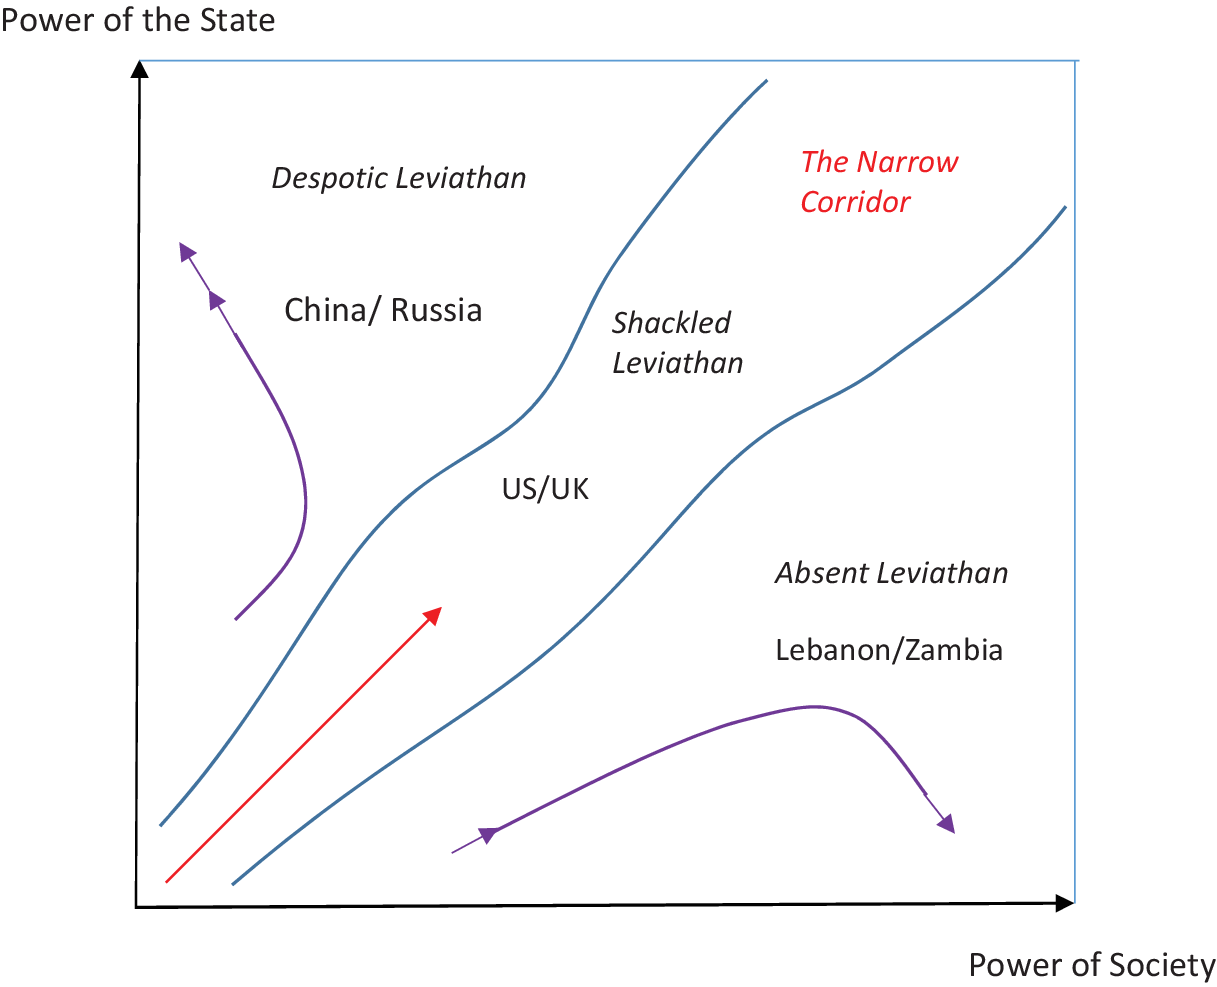
\includegraphics[width=0.7\textwidth]{Imagens Slides/i1a5.png}
    \caption{O “corredor estreito” (Acemoglu/Robinson).}
\end{figure}

\subsection{\textbf{Os movimentos regionais pré independência}}
\begin{itemize}
    \item A inconfidência Mineira (1789)
    \begin{itemize}
        \item Décadas antes do movimento já estavam presentes as ideias
liberais;
\item Portugal estabeleceu uma força excessiva na cobrança tributária e
de dívidas em 1788;
\item Cobrando mais rigorosamente diversas dívidas que ficaram
desapercebidas quando o quinto era grandioso;
\item homens ricos de Vila Rica que tinham conseguido se enriquecer bastante, reagiram, pois tais cobranças trariam descontentamento e, no limite, sua falência;

    \end{itemize}
    \item Revolução Pernambucana (1817)
    \begin{itemize}
        \item Nas bibliotecas eram fartos os autores franceses revolucionários;
        \item Houve um grande aumento dos preços, causando muito descontentamento social;
\item Movimento mais tardio, em relação à Minas, já culpava os
excessos da corte;
\item Havia muitos tributos e a emissão de moeda que custeava o governo central, causava inflação;
    \end{itemize}
\end{itemize}
\subsection{\textbf{Evidências e as razões da independência}}

\begin{figure}[H]
    \centering
    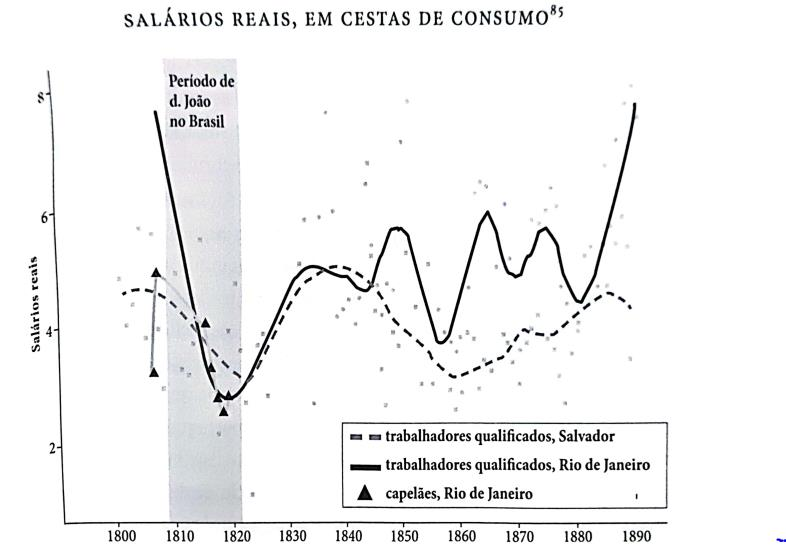
\includegraphics[width=0.5\textwidth]{Imagens Slides/i2a5.png}
    \caption{Salários reais}
\end{figure}

\begin{figure}[H]
    \centering
    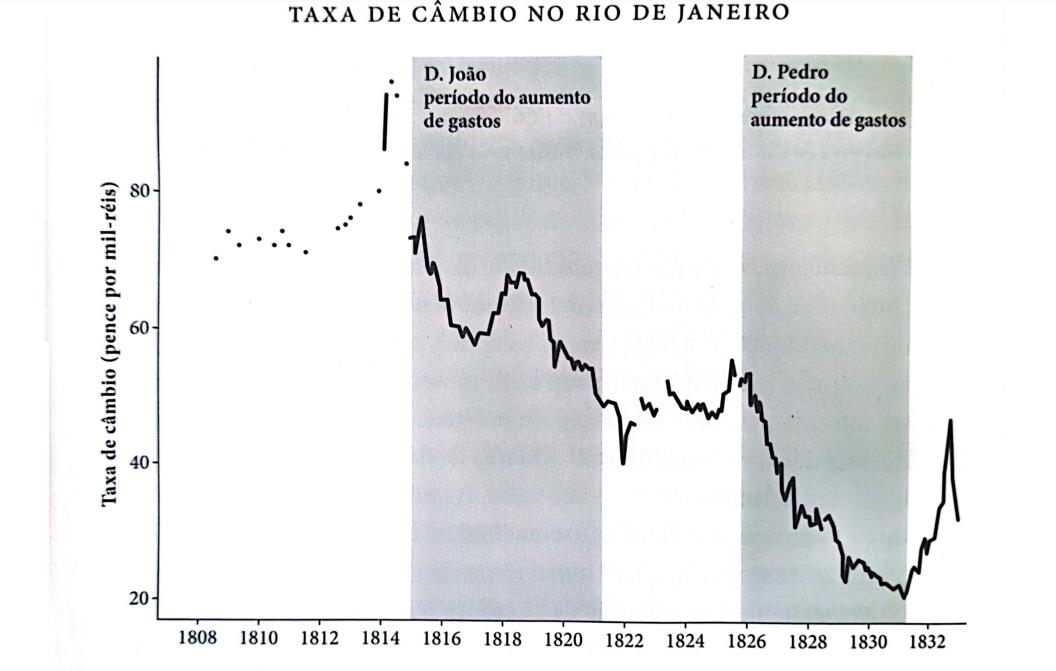
\includegraphics[width=0.5\textwidth]{Imagens Slides/i3a5.png}
    \caption{Câmbio (RJ)}
\end{figure}

\subsection{\textbf{Mentalidade X problemas econômicos}}
\begin{itemize}
    \item Nos movimentos anteriores o que pesou mais: a mentalidade ou os problemas econômicos? 
    \begin{itemize}
        \item As revoltas e os momentos de ruptura teriam como fundamental a
economia deteriorada (perda do poder de compra);
\item O descontentamento era generalizado e a piora social era atribuída à Portugal/Corte; 
\item O contexto das ideias era, em síntese, revolucionário;
\item Assim a explicação para a causa da Independência, isto é, para o fim do absolutismo, deriva da combinação entre a mentalidade e as dificuldades econômicas.
    \end{itemize}
\end{itemize}
\subsection{\textbf{Antecedentes em Portugal}}
\subsection{\textbf{Desdobramentos da Revolução de Porto}}
\begin{itemize}
    \item A Revolução Liberal do Porto (1820)
    \begin{itemize}
        \item Implementar uma monarquia constitucional em Portugal;
        \item Com o fim do Absolutismo, há uma disputa intensa pelos poderes do Rei;
\item As contas públicas foram reveladas e os desequilíbrios eram fortes;
\item Existiam muitos atrasados a pagar (Exército e outros);
\item Portugal passa a tentar tomar crédito e culpa o Brasil e sua corte repleta de privilegiados; Exigem a volta de D. João VI;
\item No Brasil, o desequilíbrio fiscal também era forte.
    \end{itemize}
\end{itemize}
\subsection{\textbf{Desdobramentos da Revolução de Porto}}
\begin{itemize}
    \item Há interesses regionais divergentes, disputas entre Lisboa, RJ, BA e
PER;
\item Lisboa pretende se aproveitar do Brasil, retomando a acumulação
financeira com tributos;
\item D. Pedro I se associa à burocracia doméstica para evitar a derrocada
econômica do RJ;
\item BA e PER, mesmo muito críticos à Corte, não concordavam com o rumo ditado por Lisboa;
\item D. Pedro I acenou em conjunto com RJ e Sul, a intenção de propor uma Constituição brasileira;
\item A lógica era atrair o apoio do Nordeste e fortalecer o Brasil diante de
Portugal.
\end{itemize}
\subsection{\textbf{Consequências no Brasil}}
\begin{itemize}
    \item A ação de D. Pedro I fomenta a formação de uma coalizão nacional em
1822, opositora à Lisboa
\begin{itemize}
    \item Uma Constituição local trouxe a perspectiva de que todas as regiões teriam representantes no Parlamento;
    \item Uma constituição única Portugal/Brasil deixava os interesses brasileiros com representação pequena;
\item Haveria maior igualdade/justiça na disputa pelo orçamento

\end{itemize}
\item Assim, votando no Parlamento, poderiam atuar mais fortemente sobre
criar/barrar tributos, por exemplo.
\begin{itemize}
    \item A carta brasileira teria sido “o motivo” para a não fragmentação do Brasil?
    \item Algumas visões: Furtado (Ouro); Prado Jr (Café); Alencastro (Tráfico).
\end{itemize}
\end{itemize}
\subsection{\textbf{Independência e Crise fiscal}}
\begin{itemize}
    \item O fim do Absolutismo vem acompanhado de um ambiente
econômico grave: crise fiscal e inflação
\item De fato: 
\begin{itemize}
    \item A crise fiscal é uma das causas do fim do Absolutismo, por que?
    \item O poder absoluto do Rei é causador da crise fiscal e, portanto, do
desagrado social (inflação, salários atrasados, excesso de tributos, sensação de não participação);
\item  A mentalidade justifica e motiva a insatisfação, a busca por mudanças bem como fornece uma direção;
\item A crise fiscal explica o fim do Absolutismo, isto é, a Independência do
Brasil.
\end{itemize}
\end{itemize}
\subsection{\textbf{Desdobramentos da Independência do Brasil}}
\begin{itemize}
    \item O fim do Absolutismo trouxe uma série de transformações institucionais que moldariam a trajetória brasileira nas décadas seguintes ao 7 de setembro de 1822:

\end{itemize}
“Para deixar de pagar suas dívidas e obter empréstimos forçados de seus súditos, a solução encontrada no Brasil foi a de um arranjo institucional que limitava a possiblidade da Coroa de conduzir unilateralmente a sua política fiscal”

“Uma vez que a câmara baixa do Parlamento era eleita, ela tornava-se
sensível aos interesses da elite com direito a voto. Essas instituições políticas formais constrangeram e em última instância eliminaram a habilidade do monarca de decidir unilateralmente sobre a cobrança de impostos, os gastos e a desvalorização da moeda.” (Summerhill no livro Inglorious Revolution.)
\begin{itemize}
    \item A mudança institucional moldou uma certa trajetória de endividamento:
    \begin{itemize}
        \item  Brasil formou boa reputação enquanto devedor; 
        \item Proporcionou que as condições de empréstimo externo fossem boas, por exemplo, com juros baixos;
        \item Também favoreceu a emissão de sua dívida interna.
    \end{itemize}
\end{itemize}
\newpage
\section{\textbf{Aula 6 - Impactos Macro e Micro do processo de Independência}}

\subsection{\textbf{Introdução}}
\begin{itemize}
    \item Brasil independente:
    \begin{itemize}
        \item cenário de baixo crescimento econômico
        \item não há industrialização no século XIX
    \end{itemize}
    \item Pontos de vista: 
    \begin{itemize}
        \item Caio Prado Jr (HEB, cap. 14)
        \item Haber e Klein (Economic Consequences of Brazilian Independence, in How Latin America Fell Behind)
        \item Furtado (FEB, cap. 17)
    \end{itemize}
\end{itemize}
\subsection{\textbf{Contexto}}
\begin{itemize}
    \item Declínio do Antigo Sistema Colonial (2ª metade séc. XVIII) 
    \begin{itemize}
        \item consolidação do capitalismo industrial
        \item necessidade crescente de acessar novos mercados
        \item luta contra a instituição monopólio (condenação dos
impérios ibéricos fundados nesta estrutura)
\item Isso quer dizer, novo contexto econômico!
\item mas permanece o escravismo
    \end{itemize}
    \item Declínio português 
    \begin{itemize}
        \item marinha decadente (contrabando cresce)
        \item compromete papel de ser metrópole 
    \end{itemize}
\item  Transferência da corte portuguesa para a colônia 
\begin{itemize}
    \item auxílio da Inglaterra
    \item RJ transforma-se em sede da monarquia com uma grande estrutura montada 
    \item “rompimento” de laços com a metrópole (posse francesa)
\end{itemize}
\end{itemize}
\subsection{\textbf{Chegada da Corte (reflexos)}}
\begin{itemize}
    \item Medidas e efeitos (aspecto institucional)
    \begin{itemize}
        \item abertura dos portos;
        \item Tratados de comércio;
        \item revogação da lei que proíbe produção de manufaturas;
        \item infraestrutura: construção de estradas, portos;
        \item estímulos para atividades econômicas no Brasil (maior intercâmbio, fixação da corte, atração do
comércio das colônias espanholas). 
Quais consequências são esperadas no balanço de pagamentos?
    \end{itemize}
\end{itemize}
\subsection{\textbf{Impactos Macro (BP}}
\begin{itemize}
    \item Chegada da corte: 
    \begin{itemize}
        \item crescem EX e IM (aumenta intercâmbio comercial e consumo doméstico); 
        \item geração de déficits comerciais crescentes.
    \end{itemize}
    \item Problema: compromissos externos futuros (amortização, pagamentos de juros etc.)
    \begin{itemize}
        \item fatores potenciais para desequilíbrio do BP;
        \item dependência de um fluxo regular de capitais estrangeiros.
    \end{itemize}
    \item Qual a tendência? 
    \begin{itemize}
        \item volatilidade da taxa de câmbio (pressão para desvalorização ) 
    \end{itemize}
    \item Consequência? 
    \begin{itemize}
        \item incerteza macroeconômica. (Furtado) O que isso quer dizer?

 
    \end{itemize}
\end{itemize}
\subsection{\textbf{Impactos Macro (Fiscal)}}
\begin{itemize}
    \item Desequilíbrio das finanças públicas (Gastos) 
    \begin{itemize}
        \item grande aparato administrativo, repartições e serviços para a corte;
        \item muitos funcionários dependentes direta e indiretamente da corte;
        \item baixa eficiência administrativa (grande desperdício e burocracia privilegiada).
    \end{itemize}
    \item Desequilíbrio das finanças públicas (Receitas) 
    \begin{itemize}
        \item arrecadação insuficiente;
        \item Brasil herda administração decadente portuguesa (não se adapta);
        \item população pequena e dispersa, dificultando arrecadar;
        \item 40\% da receita para serviço da dívida em meados do século XIX.
    \end{itemize}
    \item Déficits orçamentários estruturais 
    \begin{itemize}
        \item atrasos nos pagamentos de dívidas e salários;
    \end{itemize}
• Financiamento?
\begin{itemize}
    \item emissões de papel-moeda;
\end{itemize}
\begin{itemize}
    \item empréstimos externos;
\end{itemize}
• Resultados
\begin{itemize}
    \item Política fiscal desacreditada, volatilidade da taxa de câmbio, inflação
\end{itemize}
\begin{itemize}
    \item  incerteza macroeconômica (Furtado)
\end{itemize}

 

\end{itemize}
\subsection{\textbf{Impactos Macro (Indústria nacional)}}
\begin{itemize}
    \item Existem atividades rudimentares de manufatura com peso global pequeno
    \item Baixas tarifas comerciais:
    \begin{itemize}
        \item inviabilizam concorrência com importados (rigidez colonial substituída pela liberdade comercial)
    \end{itemize} 
    \begin{itemize}
        \item entrave para o desenvolvimento da produção nacional\end{itemize}
\end{itemize}
\textbf{Conclusão Prado Jr:} Prevalece especialização no setor exportador agrícola, similar ao sistema colonial.
\subsection{\textbf{Haber e Klein}}
\begin{itemize}
    \item Haber e Klein questionam Prado Jr:
    \begin{itemize}
        \item o comércio externo prejudicou o Brasil?
        \item Brasil era dependente da Inglaterra?
        \item o que gerou o baixo crescimento econômico?
    \end{itemize}
    \item Haber e Klein 
    \begin{itemize}
        \item o comércio externo beneficia o Brasil! 
        \item a Inglaterra não é o único parceiro comercial.
    \end{itemize}
\end{itemize}

\subsection{\textbf{Comércio}}
\begin{itemize}
    \item Não há alteração da direção e da quantidade do comércio Brasil e Inglaterra
    \begin{itemize}
        \item ocorre aumento do comércio (diversificação dos parceiros comerciais, por exemplo EUA)
        \item não significa aumento da dependência em relação a Inglaterra
        \item exportações britânicas têm pequeno impacto sobre o crescimento das importações brasileiras
    \end{itemize}
\end{itemize}
\subsection{\textbf{Comércio (conclusão)}}
\begin{enumerate}
    \item Elite brasileira não era formada por “bonecos” 
    \begin{enumerate}
        \item há persistência da escravidão
        \item  1844 dobram as taxas de importação, mas o motivo é fiscal
    \end{enumerate}
    \item Termos de Troca para o Brasil melhoram no século XIX
    \begin{enumerate}
        \item aumento PEX e queda PIM
        \item Qual a intuição econômica para explicarmos a evolução desses preços ao longo do século XIX?
        \item  ou seja, a liberdade comercial trouxe melhorias
    \end{enumerate}
\end{enumerate}
\subsection{\textbf{Manufatura Nacional}}
\begin{itemize}
    \item Haber e Klein: 
    \begin{itemize}
        \item há evidências de que o baixo crescimento econômico se deve a fatores internos e não ao regime de baixas tarifas

    \end{itemize}
    \item Lado da oferta 
    \item Para iniciar a atividade existem altos custos (60\% superior)
    \begin{itemize}
        \item Máquinas devem ser importadas
        \item alto custo de transporte
        \item salários são elevados para técnicos estrangeiros
    \end{itemize}
    \item Mobilizar capital é difícil 
    \begin{itemize}
        \item mercado de crédito primitivo, não há intermediação financeira 
    \end{itemize}
\end{itemize}

Portanto, capital próprio determina crescimento pequeno e concentrado 
\begin{itemize}
    \item Lado da demanda 
    \begin{itemize}
        \item altos custos de transporte (mulas)
        \item renda rural altamente concentrada 

    \end{itemize}

Desse modo, não permite o desenvolvimento de um mercado integrado e com participação ampla de consumidores 

    \item Conclusão: Dependência do Brasil com a Inglaterra não foi a causa do atraso industrial, fatores internos são mais importantes
    \begin{itemize}
        \item discordam de Prado Jr
        \item foco da análise é microeconômica 
    \end{itemize}
\end{itemize}
\subsection{\textbf{O que aprendemos?}}
\begin{itemize}
    \item Explicar e refletir sobre o crescimento econômico baixo brasileiro e sua industrialização atrasada
    \item  Como fazer essa reflexão?
\begin{itemize}
    \item identificar os contextos micro e macro
    \item avaliar as consequências desses contextos
    \item  construir hipóteses a partir das bases de dados
    \item aplicar e implementar modelos econométricos para estimar uma medida de incerteza macroeconômica ao longo do tempo (checar empiricamente a visão de Furtado)
\item construir de forma crítica uma explicação para o baixo crescimento econômico nesse período histórico
\end{itemize}
\end{itemize}
\newpage
\section{\textbf{Aula 7 - Formação da Economia cafeeira e a mão de obra}}
\subsection{\textbf{Introdução}}
\begin{itemize}
    \item O que é importante? 
    \begin{itemize}
        \item Explicar a formação e o crescimento da economia cafeeira ao longo do séc. XIX;
\item Identificar o problema da mão de obra e explicar como ele foi resolvido
    \end{itemize}
    \item Contexto: grande crescimento econômico internacional (UK e EUA):
    \begin{itemize}
        \item procura por novos mercados e aumento da demanda por produtos primários
        \item desorganização de algumas regiões coloniais exportadoras de primários
        \item aumento do comércio internacional
    \end{itemize}
\item Brasil 
\begin{itemize}
    \item contextos macro e micro dificultam
industrialização
\item chance: participar do comércio internacional, mas como?
\item açúcar: mercado inglês (colônias antilhanas); EUA (Cuba); beterraba (Europa)
\item algodão: domínio americano gerando queda de preços (baixa rentabilidade no Brasil); certa
prosperidade com a Guerra de Secessão
\item outros (fumo, couro, cacau) eram produtos menores
\end{itemize}
\end{itemize}
\subsection{\textbf{Café (gestação)}}
\begin{itemize}
    \item Século XVIII 
    \begin{itemize}
        \item consumo local na colônia;
        \item desorganização do Haiti, um grande produtor (gera ↑p);
        \item entrada de novos produtores na América e na Ásia.
    \end{itemize}
    \item Século XIX 
    \begin{itemize}
        \item há elevação do preço e, consequente, melhoria dos termos de troca do Brasil no início deste século;
\item supera exportações do algodão e de açúcar nos anos 1830;
\item produção cresce forte na sequência, consolidando a oferta brasileira entre as maiores do mundo.
    \end{itemize}
\end{itemize}

\begin{figure}[H]
    \centering
    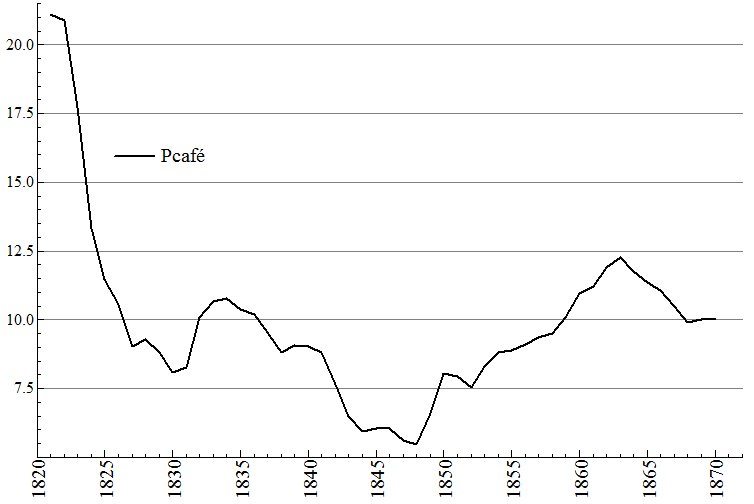
\includegraphics[width=0.7\textwidth]{Imagens Slides/i1a7.png}
    \caption{Preço internacional, cotação no mercado norte americano}
\end{figure}

\subsection{\textbf{Economia cafeeira (preços e recursos)}}
\begin{itemize}
    \item Há redução dos preços no período 1820/40, mas a produção brasileira aumenta 5x!

\end{itemize}

\begin{figure}[H]
    \centering
    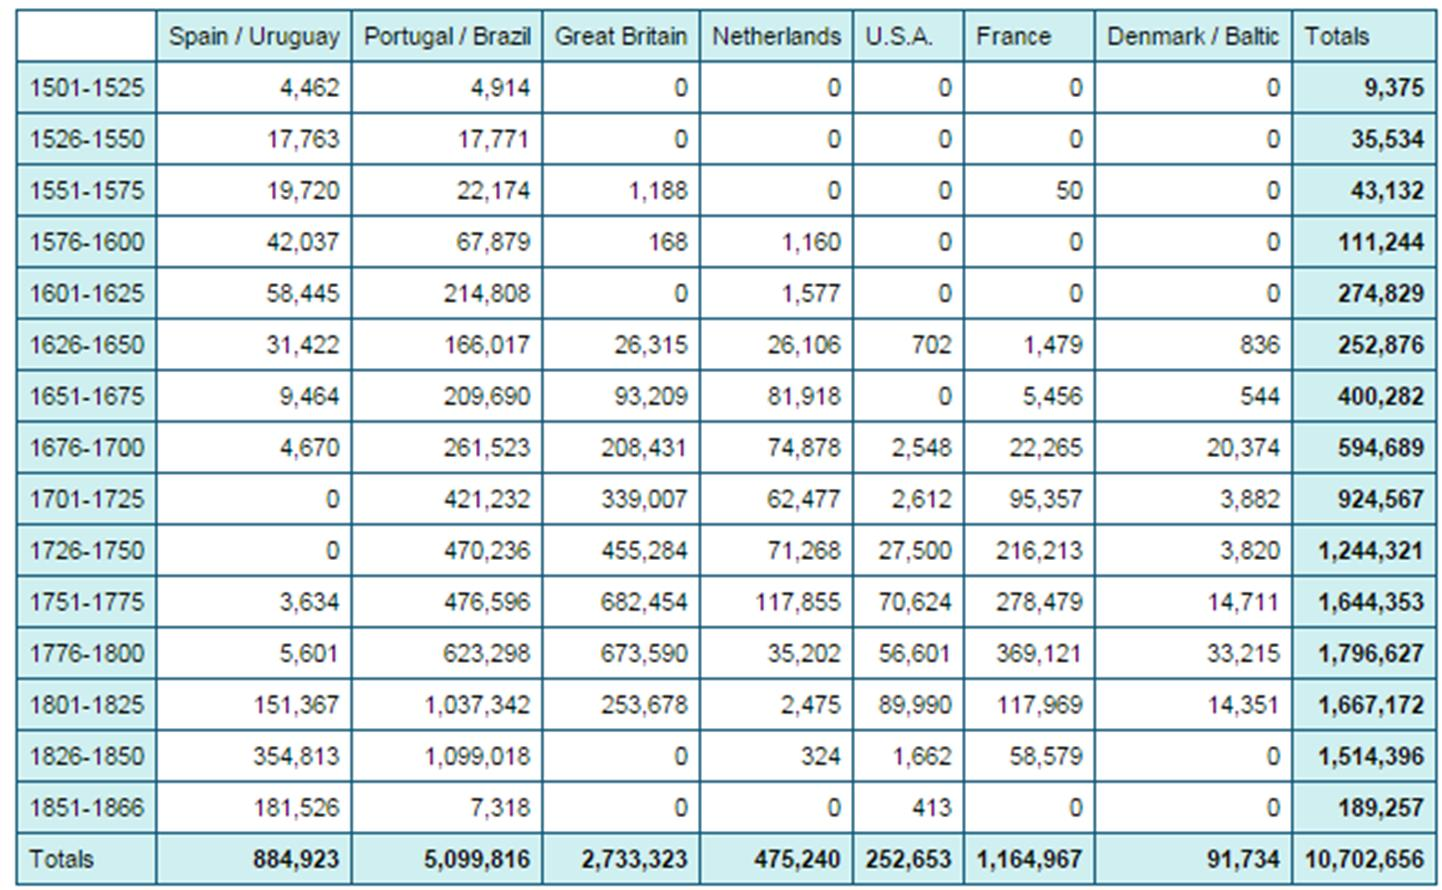
\includegraphics[width=0.7\textwidth]{Imagens Slides/i2a7.png}
    \caption{Desembarque de escravos}
\end{figure}

Como explicar essa relação? 
\begin{itemize}
    \item Celso Furtado 
    \begin{itemize}
        \item fazendas próximas ao porto RJ;
        \item necessidade de K é menor (em relação ao açúcar);
        \item há recursos ociosos (mão de obra) da economia mineira decadente.
    \end{itemize}
    \item Visão crítica 
    \begin{itemize}
        \item mas a economia mineira colapsou?
        \item o que mostra o mercado de trabalho?
        \item o grande volume de importações de escravos sustenta o aumento da produção cafeeira
    \end{itemize}
\item Consolidação da economia cafeeira ocorre em 1850-70
\item Como explicar? 
\begin{itemize}
    \item recuperação dos preços do café;
    \item preços do açúcar em baixa;
    \item há terras disponíveis e férteis; houve melhoria do transporte oceânico; nova variedade de cafeeiros. Em conjunto, melhoram a produtividade do escravo a partir de 1850 (David Eltis);
    \item café recebe investimentos de comerciantes locais.
\end{itemize}
\item Há formação de uma nova classe social 
\begin{itemize}
    \item comerciantes locais acumularam capital com lucratividade de serviços prestados para o mercado interno na primeira metade do século XIX (Furtado)
\end{itemize}
\item Consolidação da economia cafeeira: 1850-70 
\begin{itemize}
    \item nova classe: há visão de conjunto da produção e do comércio (contrário ao açúcar)
    \item atividade política: cafeicultores defendem interesses com objetivos de melhorar a atividade econômica
\end{itemize}
\item Fim da década de 1870 
\begin{itemize}
    \item economia cafeeira com condições plenas de autofinanciamento
    \item crescimento em extensão (ampliar fatores de produção)
    \item problema: mão de obra
\end{itemize}
\end{itemize}
\subsection{\textbf{Problema da mão de obra}}
\begin{itemize}
    \item Alta mortalidade e baixa natalidade dos escravos
    \begin{itemize}
        \item condições desfavoráveis de alimentação e de trabalho
    \end{itemize}
    \item Proibição do tráfico internacional de escravos (1850)
    \begin{itemize}
        \item fim da importação de escravos, resta somente o tráfico interno
    \end{itemize} 
\item Elevação dos preços dos escravos e redução do abastecimento
\begin{itemize}
    \item induz proprietários de escravos a melhorarem as condições de vida, mas população cai
\end{itemize}
\begin{itemize}
    \item intensificação da utilização, portanto, maior desgaste
\end{itemize}
\item Solução interna?
\item Oferta interna (zona rural): subsistência?
\begin{itemize}
    \item concentração fundiária (existem pessoas na subsistência, mas com alto grau de subordinação) – forte laço social
\end{itemize} 
\begin{itemize}
    \item baixa concentração demográfica (exceto sul Minas)
\end{itemize}
\item Oferta interna (zona urbana): subsistência?
\begin{itemize}
    \item maior densidade populacional (sem ocupação permanente em muitas vezes)
\end{itemize} 
\begin{itemize}
    \item problema na adaptação à disciplina do trabalho e a grande lavoura
\end{itemize}
\item Problema do transporte: há baixa mobilidade das pessoas no território brasileiro (N. Leff)

\textbf{Conclusão: a solução é externa. Como?}

\item 1ª tentativa: incentivos oferecidos pelo governo
\begin{itemize}
    \item não há mercado interno e leis são inadequadas/insuficientes
\end{itemize}
\begin{itemize}
    \item evolução para condições precárias (propaganda negativa)
\end{itemize}
\item Parcerias
\begin{itemize}
    \item renda incerta do colono (função da colheita)
\end{itemize}
\begin{itemize}
    \item pós 60, sistema misto (recebia um salário anual fixo e outra parte dependente da colheita, mas há gastos com viagem)
\end{itemize}
\item Pós 70
\begin{itemize}
    \item  governo responsabiliza-se pelo transporte
\end{itemize}
\begin{itemize}
    \item fazendeiro com os custos do 1ª ano e dispor terras para subsistência
\end{itemize}

Essas foram as condições de demanda por trabalhadores, mas não foram suficientes
\item Lado da Oferta (unificação política Italiana)
\begin{itemize}
    \item desorganização da região sul gera problemas sociais no norte
\end{itemize}
\begin{itemize}
    \item Solução Italiana? Incentivar migração
\end{itemize}
\item Fluxo para o Brasil
\begin{itemize}
    \item 1870: 13 mil;1880: 184 mil;1890: 609 mil
\end{itemize}
\item Combinação de fatores para solução externa :
\begin{itemize}
    \item Estado + Fazendeiros (internos)
\end{itemize}
\begin{itemize}
    \item Unificação italiana (externo)
\end{itemize}
\item \textbf{Resultado:} corrente migratória significativa de origem europeia para as grandes plantações de café
\end{itemize}
\subsection{\textbf{Conclusão}}
\begin{itemize}
    \item O que aprendemos e quais eram os objetivos?
    \begin{itemize}
        \item  explicar a dinâmica da consolidação do café
    \end{itemize}  
    \begin{itemize}
        \item explicar porque a mão de obra torna-se problema
    \end{itemize}
    \begin{itemize}
        \item identificar dificuldades para a solução deste problema
    \end{itemize}
    \begin{itemize}
        \item entender e explicar a importância do tráfico de escravos para a formação econômica do Brasil
    \end{itemize} 
    \begin{itemize}
        \item construir, a partir dos pontos acima, o novo contexto econômico brasileiro formado
    \end{itemize}
\end{itemize}
\newpage

\section{\textbf{Aula 8 - Estradas de Ferro}}
\subsection{\textbf{Introdução}}
\begin{itemize}
    \item Construção das estradas de ferro significa substituir o antigo sistema de transporte (tropa de animais)
    \item Anos 1830: aparato legal autoriza concessão desse serviço de transporte
    \begin{itemize}
        \item   privilégios e garantias para a construção de linhas férreas;
    \end{itemize}
    \begin{itemize}
        \item mas não há perspectivas claras da rentabilidade nesse período
    \end{itemize}
    \item 1865 e 1867: 1as ferrovias (SP-RJ e Santos- Jundiaí)
    \item Efeitos e impactos econômicos esperados?
\end{itemize}
\subsection{\textbf{Café e ferrovias}}
\begin{itemize}
    \item Há forte ligação entre os dois componentes
    \begin{itemize}
        \item  café segue para o interior paulista
    \end{itemize}
    \begin{itemize}
        \item o estado das estradas de rodagem é péssimo
    \end{itemize}
    \begin{itemize}
        \item necessidade das ferrovias para essa expansão
    \end{itemize}
    \begin{itemize}
        \item há relação direta entre rede ferroviária, exportação de café e habitantes
    \end{itemize}
    \item Gera efeitos além de melhorias de transportar café até o porto
    \begin{itemize}
        \item desenvolve e diversifica a economia
    \end{itemize}
    \begin{itemize}
        \item  Estradas de ferro foram modelos de empresa para outros setores
    \end{itemize}
    \begin{itemize}
        \item grande crescimento populacional (relativo a outras capitais)
    \end{itemize}
\end{itemize}
\subsection{\textbf{São Paulo e ferrovias}}
\begin{itemize}
    \item  Os cafeicultores, a partir de grande acumulação de capital:
    \begin{itemize}
        \item investem em estradas de ferro
    \end{itemize}
    \item As estradas de ferro possibilitam moradia dos “Barões de Café” na cidade de São Paulo
    \begin{itemize}
        \item demanda por serviços municipais cresce;
    \end{itemize}
    \begin{itemize}
        \item há melhoria dos serviços públicos;
    \end{itemize}
    \begin{itemize}
        \item esses dois itens favorecem a urbanização;
    \end{itemize}
    \begin{itemize}
        \item acionistas ferroviários têm grande participação nesses investimentos.
    \end{itemize}
\end{itemize}
\subsection{\textbf{Ferrovias e diversificação}}
\begin{itemize}
    \item Ferroviário e comerciantes (década de 1880)
    \begin{itemize}
        \item participam em conjunto, ofertando serviços públicos (transporte urbano, gás, água/esgoto)
    \end{itemize}
    \begin{itemize}
        \item grande parte da renda gerada em atividades não-agrícolas (Formação do Grande Capital Cafeeiro)
    \end{itemize}
    \item Ou seja, há diversificação de investimentos
\end{itemize}
\subsection{\textbf{Anos 1890}}
\begin{itemize}
    \item  Efeitos da consolidação da imigração geram novas perspectivas de investimentos
    \begin{itemize}
        \item  aumento da população
    \end{itemize}
    \begin{itemize}
        \item mercado interno consumidor
    \end{itemize}
    \begin{itemize}
        \item novos hábitos de consumo
    \end{itemize}
    \begin{itemize}
        \item criação do mercado de trabalho urbano (atrai certa quantidade de imigração espontânea)
    \end{itemize}
    \item Esses efeitos geram um novo contexto econômico
    \begin{itemize}
        \item estimula investimento
    \end{itemize}
    \begin{itemize}
        \item novo potencial de crescimento econômico!
    \end{itemize}
\end{itemize}
\subsection{\textbf{Capital nacional e Estrangeiro}}
\begin{itemize}
    \item No final dos anos 80, SP constitui um polo de atração de capital estrangeiro
    \item Agentes nacionais enfrentam forte concorrência
    \begin{itemize}
        \item diminui o controle do capital cafeeiro sobre as principais atividades
    \end{itemize}
    \begin{itemize}
        \item buscam novas regiões (interior) e novas atividades (empreendimentos imobiliários)
    \end{itemize}
\end{itemize}
\subsection{\textbf{Conclusão}}

\begin{itemize}
    \item Porque estudamos? O que aprendemos?
    \begin{itemize}
        \item  identificar e explicar a melhoria dos fatores internos (eram restrições de acordo com Haber/Klein)
    \end{itemize}
    \begin{itemize}
        \item  interpretar os efeitos da diversificação e desenvolveras consequências para nossa formação econômica.
    \end{itemize}
\end{itemize}
\newpage

\section{\textbf{Aula 9 - Política econômica e problemas econômicos no período de 1870-1889}}
\subsection{\textbf{Introdução}}
\begin{itemize}
    \item O que é importante?
    \begin{itemize}
        \item Discutir os cenários econômicos desse período histórico;
    \end{itemize}
    \begin{itemize}
        \item Refletir sobre os comportamentos do setor externo, da gestão fiscal e monetária, notando que eles influenciam a dinâmica do mercado de câmbio
    \end{itemize}
    \item Antes uma breve retomada do contexto de 1822-1870
\end{itemize}
\subsection{\textbf{1822-1845}}
\begin{itemize}
    \item  Contexto de ajustes, correções e esforço para evitar a fragmentação do
Império
\begin{itemize}
    \item Fortes gastos militares (maior peso nas despesas);
\end{itemize}
\begin{itemize}
    \item Desequilíbrios fiscais fortes e empréstimos externos;
\end{itemize}
\begin{itemize}
    \item  Houve grande expansão da oferta monetária;
\end{itemize}
\begin{itemize}
    \item Setor agrícola era central, enquanto mineração e indústria eram marginais;
\end{itemize}
\begin{itemize}
    \item A balança comercial mostrou comportamento padrão deficitário;
\end{itemize}
\begin{itemize}
    \item Investimento estrangeiro ocupa papel modesto nesse contexto. Os empréstimos são relevantes;
\end{itemize}
\begin{itemize}
    \item Há alta razão dívida externa/exportações;
\end{itemize}
\item Mercado cambial
\begin{itemize}
    \item Mostrou uma tendência de desvalorização da moeda ao longo do tempo;
\end{itemize}
\begin{itemize}
    \item Ademais, mostrou diversos picos de volatilidade cambial.
\end{itemize}
\item Consequências
\begin{itemize}
    \item A depreciação tendeu a favorecer os exportadores, mas elevou  custo de vida da população ao encarecer os importados;
\end{itemize}
\begin{itemize}
    \item Como parte da dívida pública era em moeda estrangeira, houve deterioração fiscal;
\end{itemize}
\begin{itemize}
    \item  Os vários picos de volatilidade cambial sugerem instabilidade macro elevada neste contexto histórico.
\end{itemize}
\end{itemize}
\subsection{\textbf{Em geral}}
\begin{itemize}
    \item Análise econômica do período como um todo (1822-1889)
    \begin{itemize}
        \item As escolhas (Corte e depois Império) moldaram a dinâmica fiscal;
    \end{itemize}
    \begin{itemize}
        \item Os cenários global e doméstico influenciaram o BP;
    \end{itemize}
    \begin{itemize}
        \item  Ambos os fatores, impactaram o ambiente econômico, deixando-o mais incerto ou mais previsível;
    \end{itemize}
\begin{itemize}
    \item Esta variação de cenários não é observável, mas podemos tentar obter uma medida de aproximação, estimando uma medida de incerteza (como fazer?).
\end{itemize}
\end{itemize}
\subsection{\textbf{Primeiras conclusões}}
\begin{itemize}
    \item No geral, os picos de volatilidade estiveram associados aos períodos
de deterioração fiscal
\begin{itemize}
    \item  As contas externas não suavizaram esses picos (BC foi negativa);
\end{itemize}
\begin{itemize}
    \item A política monetária, em geral, expansionista também ajuda a explicar a volatilidade;
\end{itemize}
\begin{itemize}
    \item  Assim como as instabilidades políticas;
\end{itemize}
\begin{itemize}
    \item Os momentos de depreciação cambial impactavam os compromissos da dívida externa, deteriorando o fiscal;
\end{itemize}
\begin{itemize}
    \item Com isso, a avaliação dos investidores estrangeiros e suas reações progressivamente pesam bastante nas decisões de política econômica
\end{itemize}
\end{itemize}
\subsection{\textbf{1845-1870}}
Marcas gerais
    \begin{itemize}
        \item Período modernizante: fim do tráfico transatlântico de escravos, ferrovias, expansão bancária, café. Mas o desfecho se dá com a Guerra do Paraguai.
    \end{itemize}
Características macro
\begin{itemize}
    \item Crescimento das exportações é tímido. A balança comercial persiste em seu padrão deficitário até a década de 1860; (ver Graf. slide anterior)
\end{itemize}
\begin{itemize}
    \item Cenário fiscal, no geral, apresenta melhoria e denota responsabilidade;(ver prox. slide Tab. 8.1)
\end{itemize}
\begin{itemize}
    \item As taxas de juros e os descontos dos empréstimos externos mostram declínio no pós 1850;
\end{itemize}
\begin{itemize}
    \item Em 1857 há justaposição da crise norte americana (diante de uma desaceleração global) com uma crise bancária no Brasil;
\end{itemize}
\begin{itemize}
    \item Guerra do Paraguai (1865-1870)
\end{itemize}
\begin{itemize}
    \begin{itemize}
        \item Elevou gastos (despesas militares) e houve emissão monetária para financiar;
    \end{itemize}
\end{itemize}
\begin{itemize}
    \begin{itemize}
        \item Causou depreciação cambial e “inflação”;
    \end{itemize}
\end{itemize}
\begin{itemize}
    \begin{itemize}
        \item Ainda elevou o patamar de gastos públicos, deixando um patamar maior como novo padrão.
    \end{itemize}
\end{itemize}
\subsection{\textbf{O período 1870-1889}}
\begin{itemize}
    \item Grandes marcas deste subperíodo
    \begin{itemize}
        \item abolicionismo, republicanismo e federalismo moldam a mentalidade política;
    \end{itemize}
    \begin{itemize}
        \item Brasil estreita relações e contatos com o resto do mundo
    \end{itemize}
    \begin{itemize}
        \item Grande expansão cafeeira;
    \end{itemize}
    \begin{itemize}
        \item Crescimento da malha ferroviária e fluxo populacional estrangeiro;
    \end{itemize}
    \begin{itemize}
        \item  Crescimento do setor industrial brasileiro.
    \end{itemize}
\end{itemize}
\subsection{\textbf{Gestão fiscal 1870-1889}}
\begin{itemize}
    \item No campo fiscal, as pesquisas mais recentes tendem a mostrar um período fiscal responsável no Império
    \begin{itemize}
        \item Não houve déficits fiscais sistemáticos;
    \end{itemize}
    \begin{itemize}
        \item As pioras fiscais estão associadas a episódios localizados: seca (1878) e a Guerra do Paraguai (final dos anos 1860);
    \end{itemize}
    \begin{itemize}
        \item  No geral, os resultados primários foram superavitários;
    \end{itemize}
    \begin{itemize}
        \item As condições de financiamento interno e externo tenderam a melhorar ao longo do tempo;
    \end{itemize}
    \begin{itemize}
        \item Nossa medida de volatilidade tende a suportar essa visão.
    \end{itemize}
\end{itemize}
\subsection{\textbf{Discussões sobre a oferta monetária}}
\begin{itemize}
    \item A oferta de moeda era limitada nos tempos do Império, mesmo nas regiões mais importantes houve episódios de escassez
    \begin{itemize}
        \item prevaleceu o pensamento econômico metalista, no qual excessos monetários geravam deterioração econômica;
    \end{itemize}
    \begin{itemize}
        \item  de fato, o Brasil conviveu com uma séria restrição de liquidez e de crédito. Houve crises e episódios de falências bancárias. O mercado era primitivo e pouco elástico;
    \end{itemize}
    \begin{itemize}
        \item vigorava um certo ciclo no qual situações que exigiam maior oferta, eram pontualmente resolvidas e, por vezes, gerava queda do valor da moeda;
    \end{itemize}
    \begin{itemize}
        \item O ciclo se fechava com a retomada do debate econômico pelos metalistas e novas medidas restritivas.
    \end{itemize}

 
\end{itemize}
\subsection{\textbf{Instituições e mercado de crédito}}
\begin{itemize}
    \item Mudanças institucionais tenderam a impedir o desenvolvimento do mercado de crédito e de capitais, dificultando o crescimento econômico.
    \begin{itemize}
        \item tal como apontaram Haber e Klein;
        \item exemplo: Lei nº 1.083 de 22 de agosto de 1860 - Lei dos entraves;
        \item Essa lei limitou a emissão dos bancos e exigiu que a criação de novos bancos de depósito fossem autorizados somente pelo aval do legislativo;
        \item Isso tendeu a deixar o mercado bancário concentrado, com oferta menor de crédito, resultando em taxas de juros elevadas;
        \item mais modernamente pesquisas indicam que o mercado de crédito precário penaliza a PTF, isto é, o crescimento de longo prazo de uma economia;
    \end{itemize}
    \item Assim, o problema no mercado monetário foi mais a escassez do que o excesso.
    \item Portanto: ajuda a explicar o baixo crescimento econômico do período.
\end{itemize}
\subsection{\textbf{Discussões sobre o câmbio}}
\begin{itemize}
    \item O Brasil não operava o padrão-ouro, apesar de ter uma “paridade desejada”. Isto é, o câmbio era flutuante!
    \item Câmbio considerado como um bom “termômetro” da “saúde econômica”.
    \item Determinantes do câmbio
    \begin{itemize}
        \item  No Império predominava o pensamento metalista – câmbio é determinado pela quantidade de moeda;
    \end{itemize}
    \begin{itemize}
        \item Mas para os papelistas, o que determinava o câmbio era a balança comercial (na verdade, o BP);
    \end{itemize}
    \begin{itemize}
        \item O que explicaria a depreciação de 1875 até 1886? Oferta monetária ou BP?
    \end{itemize}
    \begin{itemize}
        \item Crescimento monetário bastante modesto; (Villela)
    \end{itemize}
    \begin{itemize}
        \item Mas o BP parece mostrar tendência de deterioração e em termos relativos menor disponibilidade de libras ao longo desse período;
    \end{itemize}
    \begin{itemize}
        \item e como foi suave não gerou pico de volatilidade, mas a queda de oferta de libras pode ter sido sim suficiente para explicar a depreciação (diferentemente do que coloca Villela).
    \end{itemize}
\end{itemize}
\subsection{\textbf{O setor externo (1870-1889)}}
\begin{itemize}
    \item  As evidências do setor externo neste período foram produzidas pela pesquisa
de Gustavo Franco e estão disponíveis no Ipeadata
\begin{itemize}
    \item Elas mostram grandes oscilações ao longo do tempo e tenderam a gerar períodos instáveis no mercado de câmbio;
\end{itemize}
\begin{itemize}
    \item Essas oscilações são marcantes na conta de capital e no saldo da balança
\end{itemize}
comercial, inclusive há grande variação no preço do café;
\begin{itemize}
    \item Franco atribui que, potencialmente, uma mudança nos fluxos de capitais estrangeiros tende a gerar movimento no câmbio (pode, por exemplo, explicar a depreciação de 1875-1886, em oposição ao que coloca Villela);
\end{itemize}
\begin{itemize}
    \item Uma deterioração conjunta da BC e da BK em 1886 pode ajudar a explicar um certo aumento da volatilidade cambial observado no final do Império.
\end{itemize}
\end{itemize}
\subsection{\textbf{Grandes conclusões para 1822-1889}}
\begin{itemize}
    \item Escolhas de política econômica e suas consequências
    \begin{itemize}
        \item  Política monetária – quando foi expansionista, em muitos casos aliviava aumento da demanda por moeda (necessidade liquidez - crises bancárias e secas);
    \end{itemize}
    \begin{itemize}
        \item Assim, às vezes gerou excesso de liquidez causando depreciação cambial e inflação;
    \end{itemize}
    \begin{itemize}
        \item Mas, quando satisfazia aumentos na demanda de moeda não gerava excesso de liquidez e inflação;
    \end{itemize}  
    \begin{itemize}
        \item Vale lembrar que o sistema era precário, tendendo ele próprio a gerar crise de liquidez;
    \end{itemize}
    \begin{itemize}
        \item Política fiscal - expansionista pelo lado das despesas, mas solvente a partir da década de 1840 (escolha refletida na volatilidade do câmbio);
    \end{itemize}
    \begin{itemize}
        \item Déficits financiados com dívida externa e interna em sua maioria. Monetização foi a exceção.
    \end{itemize}
\item  Dinâmica cambial
\begin{itemize}
    \item A tendência ao longo do período foi de depreciação cambial;
\end{itemize}
\begin{itemize}
    \item No geral, portanto, incentivou os exportadores, encareceu os importados e penalizou o ambiente fiscal;
\end{itemize}
\begin{itemize}
    \item A volatilidade também chama bastante atenção mostrando diversos picos;
\end{itemize}
\begin{itemize}
    \item As escolhas de política econômica influenciaram de forma significativa o cenário brasileiro formando contextos de baixa volatilidade e de alta;
\end{itemize}
\begin{itemize}
    \item A crescente inserção brasileira no cenário externo, ao longo da segunda metade do XIX, trouxe consequências marcantes. O cenário Global passa a influenciar com relevância o cenário doméstico.
\end{itemize}
\end{itemize}
\newpage

\section{\textbf{Aula 10 - Problemas econômicos e política econômica na década de 1890}}
\subsection{\textbf{Introdução e temas importantes}}
\begin{itemize}
    \item Período: segunda metade dos 80 e década de 1890
    \item O Brasil e a Economia Internacional
    \item  Assalariamento e demanda por moeda
    \item Escolhas de Política Econômica
    \begin{itemize}
        \item embate no pensamento econômico: papelistas x metalistas
    \end{itemize}
\end{itemize}
\subsection{\textbf{Contexto}}
\begin{itemize}
    \item Doméstico
    \begin{itemize}
        \item Trabalho assalariado (imigração);
    \end{itemize}
    \begin{itemize}
        \item Economia cafeeira em forte expansão;
    \end{itemize}
    \begin{itemize}
        \item Estradas de Ferro;
    \end{itemize}
    \begin{itemize}
        \item Diversificação econômica.
    \end{itemize}
    \item Internacional
    \begin{itemize}
        \item Grandes fluxos: capitais, comércio e populacional;
    \end{itemize}
    \begin{itemize}
        \item Padrão-ouro.
    \end{itemize}
\end{itemize}
\subsection{\textbf{Brasil e a economia internacional}}
\begin{itemize}
    \item Conta Capital ganha importância
    \begin{itemize}
        \item possível suportar déficits comerciais maiores;
    \end{itemize}
    \begin{itemize}
        \item déficits seriam inviáveis na ausência dessas entradas de capitais;
    \end{itemize}
    \begin{itemize}
        \item possível compensar instabilidade temporária na receita comercial
    \end{itemize}
    \item Conclusão: permite maiores taxas de consumo e de investimento (absorção), mas há vulnerabilidade externa
    \item  Relação entre Conta Comercial e Conta Capital
    \begin{itemize}
        \item promove estabilidade macro nos países centrais ajuste: BP<0, (↓reservas internacionais), reduz oferta monetária doméstica (padrão-ouro), queda de preços,melhora os termos de troca, estimulando EX e reduzindo IM
    \end{itemize}

\begin{itemize}
    \item Ou seja, há correlação positiva entre EX de capital e termos de troca
\end{itemize}
\item No entanto, essa correlação é negativa para países periféricos. (Furtado)
\begin{itemize}
    \item como era o mecanismo de ajustamento nessa visão?
\end{itemize}
\item Como se posiciona Gustavo Franco sobre o tema?
\item Dificuldade cambial pode ser consequência de uma redução das entradas de capital
\item Dada uma depreciação cambial:
\begin{itemize}
    \item Consequências possíveis?
\end{itemize}desvalorização real da taxa de câmbio;
\item pode provocar redução do déficit comercial;
\item pode gerar um cenário de “socialização das
perdas”
\end{itemize}
\subsection{\textbf{Determinantes da taxa de câmbio}}
\begin{itemize}
    \item Visão tradicional (Furtado)
    \begin{itemize}
        \item  crises cambiais são consequências de choques comerciais (variação Pcafé).
    \end{itemize}
    \item Múltiplos fatores (Franco e Fritsch)
    \begin{itemize}
        \item fluxo de capitais (Ex.: Crise Baring);
    \end{itemize}
    \begin{itemize}
        \item alteração monetária no âmbito doméstico;
    \end{itemize}
    \begin{itemize}
        \item aumento nas IM, a partir de uma expansão de crédito ou de um cenário de crescimento econômico
    \end{itemize}
\end{itemize}
\subsection{\textbf{Crise Baring Brothers}}
\begin{itemize}
    \item A Argentina apresenta um processo de forte endividamento externo na década de 1880
    \begin{itemize}
        \item muitos investimentos de longa maturação;
    \end{itemize}
    \begin{itemize}
        \item há desconfiança dos investidores ingleses na capacidade de pagamento da Argentina;
    \end{itemize}
    \begin{itemize}
        \item há reposicionamento financeiro dos investidores e fortes prejuízos (grupo Baring Brothers quebra);
    \end{itemize}
    \begin{itemize}
        \item default da Argentina inicia crise financeira internacional e transmite efeitos.
    \end{itemize}
    \begin{itemize}
        \item  efeitos esperados no Brasil?
    \end{itemize}
\end{itemize}
\subsection{\textbf{Assalariamento}}
\begin{itemize}
    \item Altera estrutura e o potencial de acumulação de riqueza
    \begin{itemize}
        \item impacto monetário;
    \end{itemize}
    \begin{itemize}
        \item despesas com mão de obra associadas ao período de colheita;
    \end{itemize}
    \begin{itemize}
        \item  elevada e concentrada demanda por moeda (agrava com a abolição);
    \end{itemize}
    \begin{itemize}
        \item sistema bancário precário e concentrado
        \item incentiva entesouramento (baixa
propensão por depósito, reduzindo efeito
do multiplicador)
\item baixa razão encaixe/depósitos:
vulnerabilidade de liquidez
\item “inelasticidade do meio circulante”: incapacidade dos bancos contrair/expandir crédito de acordo com a necessidade
    \end{itemize}
\end{itemize}
\subsection{\textbf{Leis para emissão}}
\begin{itemize}
    \item Tentativas de solucionar a escassez de moeda
    \begin{itemize}
        \item  lei (julho 85) autoriza emissão monetária governamental para auxiliar bancos: insuficiente
    \end{itemize}
    \begin{itemize}
        \item nova conjuntura de escassez monetária (final de 86)
    \end{itemize}
    \begin{itemize}
        \item  política monetária contracionista em conflito com aumento da demanda por moeda (papelistas x metalistas)
    \end{itemize}
\end{itemize}
\subsection{\textbf{Leis para emissão e cenário econômico}}
\begin{itemize}
    \item Nov. 88 – Lei de Reforma Bancária (instituição)
    \begin{itemize}
        \item promover expansão bancária
    \end{itemize}
    \begin{itemize}
        \item novo banco de emissão (BNB) com caráter conversível no início, mas isso não se sustenta ao longo do tempo
    \end{itemize}
    \item 1888 é um ano favorável com superávit no BP e difusão do trabalho assalariado:
    \begin{itemize}
        \item perspectivas positivas de crescimento econômico
    \end{itemize}
    \begin{itemize}
        \item ao absorver divisas estrangeiras permite expansão monetária
    \end{itemize}
    \begin{itemize}
        \item concessão de créditos (auxílio a lavoura) e atender necessidades do setor bancário
    \end{itemize}
    \begin{itemize}
        \item grande e crescente expansão monetária (final de 80 e início dos 90)
    \end{itemize}
\end{itemize}
\subsection{\textbf{Política Monetária}}
\begin{itemize}
    \item Há dificuldades de adotar o padrão-ouro
nesse contexto? Porque?
\begin{itemize}
    \item agentes devem acreditar na manutenção do sistema (credibilidade)
\end{itemize}
\begin{itemize}
    \item frequentes dificuldades no BP em situação de escassez de reservas: instabilidade cambial
\end{itemize}
\begin{itemize}
    \item choque com os incentivos institucionais derivados da reforma bancária
\end{itemize}

\end{itemize}
\subsection{\textbf{Conjuntura 1890-1894}}
\begin{itemize}
    \item Ambiente externo: Moratória argentina e Crise
Baring. Efeitos esperados?
\begin{itemize}
    \item queda do fluxo de capitais e consequente movimento cambial;
\end{itemize}
\begin{itemize}
    \item forte depreciação cambial;
\end{itemize}
\begin{itemize}
    \item cresce dívida externa em moeda nacional;
\end{itemize}
\begin{itemize}
    \item ↓Pcafé depreciação cambial o que aumentam os lucros do exportador e incentiva expansão da produção de café;
\end{itemize}
\begin{itemize}
    \item  produto nacional “substitui” consumo de importados básicos;
\end{itemize}
\item Interno: agravamento do processo especulativo – cai Ministro Rui Barbosa
\begin{itemize}
    \item perda do controle governista sobre a onda especulativa;\end{itemize}
\begin{itemize}
    \item  não há normas de concessão de crédito e garantias visando o retorno desse crédito.
\end{itemize}
\begin{itemize}
    \item  ou seja, instituições incentivam a má utilização do crédito.
\end{itemize}
\item Expectativas de crescimento do fim dos 1880 são revertidas
\item  Reação: Tentativas de obtenção de empréstimo externo
\end{itemize}
\subsection{\textbf{Conjuntura 1898}}
\begin{itemize}
    \item  Pacote de Assistência financeira – Funding loan
    \begin{itemize}
        \item rolar compromissos dos serviços da dívida e garantias de juros;
    \end{itemize}
    \begin{itemize}
        \item fortes medidas de ajuste fiscal e monetário (condicionalidades do pacote);
    \end{itemize}
\begin{itemize}
    \item fiscal: melhoria administrativa, controle de despesas e aumento da pauta de produtos de consumo taxados;
\end{itemize}
\begin{itemize}
    \item monetária: forte contração do papel-moeda em circulação (parte do empréstimo entra como títulos no sistema bancário e o meio circulante correspondente é destruído).
\end{itemize}
\item Avaliação e política do Ministro Murtinho
\begin{itemize}
    \item houve excesso de emissões e de capitais ao longo da década e isso foi prejudicial;
\end{itemize}
\begin{itemize}
    \item deve imprimir seleção natural aos setores;
\end{itemize}
\begin{itemize}
    \item seguindo a doutrina metalista.
\end{itemize}
\end{itemize}
\subsection{\textbf{Conjuntura: transição dos séculos}}
\begin{itemize}
    \item Conjuntura é consequência do Funding Loan
    \begin{itemize}
        \item mercado auxilia ou agrava situações de crise de acordo com a interpretação da política econômica
    \end{itemize}
    \begin{itemize}
        \begin{itemize}
            \item  o que isso quer dizer?
        \end{itemize}
    \end{itemize}
    \begin{itemize}
        \item o pacote gera “boa imagem” e há entrada de capitais, gerando apreciação cambial
    \end{itemize}

\begin{itemize}
    \begin{itemize}
        \item consequências?
    \end{itemize}
\end{itemize}
\begin{itemize}
    \item  redução da dívida em moeda nacional
\end{itemize}
\begin{itemize}
    \item  dificuldade aos exportadores (câmbio e crédito)
\end{itemize}
\begin{itemize}
    \item sistema bancário entra em crise com redução da liquidez
\end{itemize} 
\end{itemize}
\subsection{\textbf{Conclusão: o que aprendemos e por que?}}
\begin{itemize}
    \item Aplicar conteúdo da macroeconomia para explicar e avaliar a conjuntura econômica brasileira
    \item  Identificar que múltiplos fatores determinam a taxa de câmbio
    \begin{itemize}
        \item  explicar os efeitos de uma crise externa
    \end{itemize}
    \begin{itemize}
        \item  avaliar a influência da política monetária doméstica
    \end{itemize}
\item Identificar e explicar as consequências de uma depreciação cambial nos anos 1890
\begin{itemize}
    \item entender a importância da estrutura de endividamento
\end{itemize}
\begin{itemize}
    \item notar a transmissão dos efeitos (inflação, ciclo do café, produção nacional)
\end{itemize}
\item Avaliar as opções de política econômica e as consequências observadas
\begin{itemize}
    \item explicar o papel e os efeitos de um ajuste fiscal
\end{itemize}
\begin{itemize}
    \item  avaliar o papel das expectativas
\end{itemize}
\end{itemize}

\begin{figure}[H]
    \centering
    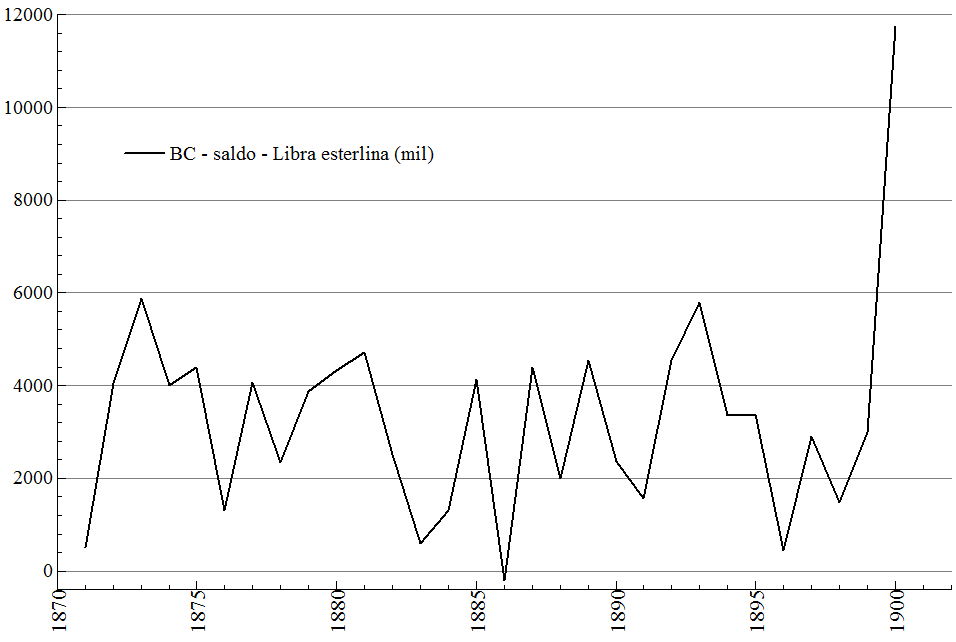
\includegraphics[width=0.5\textwidth]{Imagens Slides/i1a10.png}
    \caption{BC - Saldo - Libra esterlina (mil)}
\end{figure}

\begin{figure}[H]
    \centering
    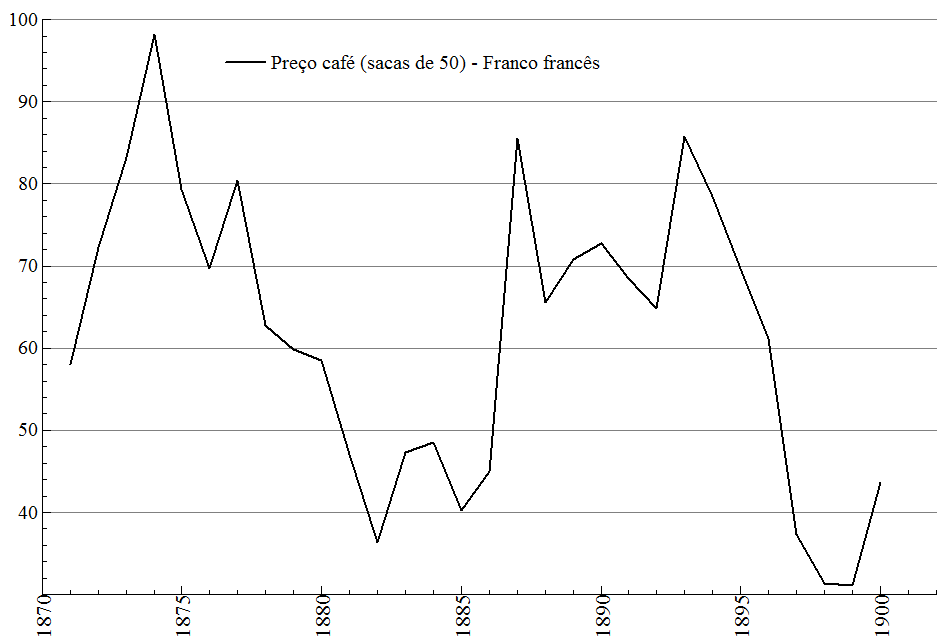
\includegraphics[width=0.5\textwidth]{Imagens Slides/i2a10.png}
    \caption{O Café no Comércio}
\end{figure}

\begin{figure}[H]
    \centering
    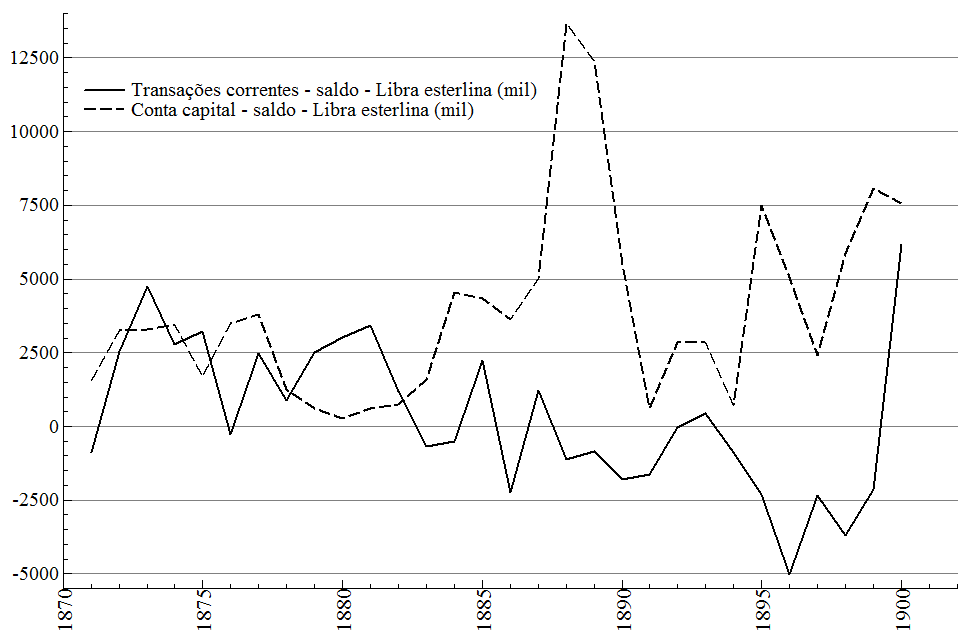
\includegraphics[width=0.5\textwidth]{Imagens Slides/i3a10.png}
    \caption{O balanço de pagamentos do Brasil, 1870-1900}
\end{figure}

\begin{figure}[H]
    \centering
    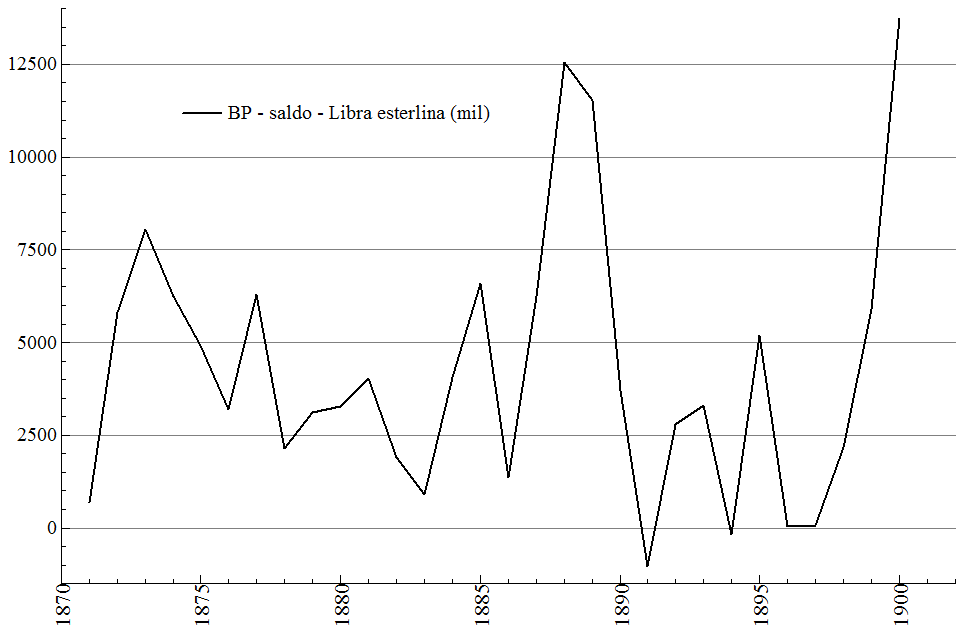
\includegraphics[width=0.5\textwidth]{Imagens Slides/i4a10.png}
    \caption{O balanço de pagamentos do Brasil, 1870-190}
\end{figure}

\begin{figure}[H]
    \centering
    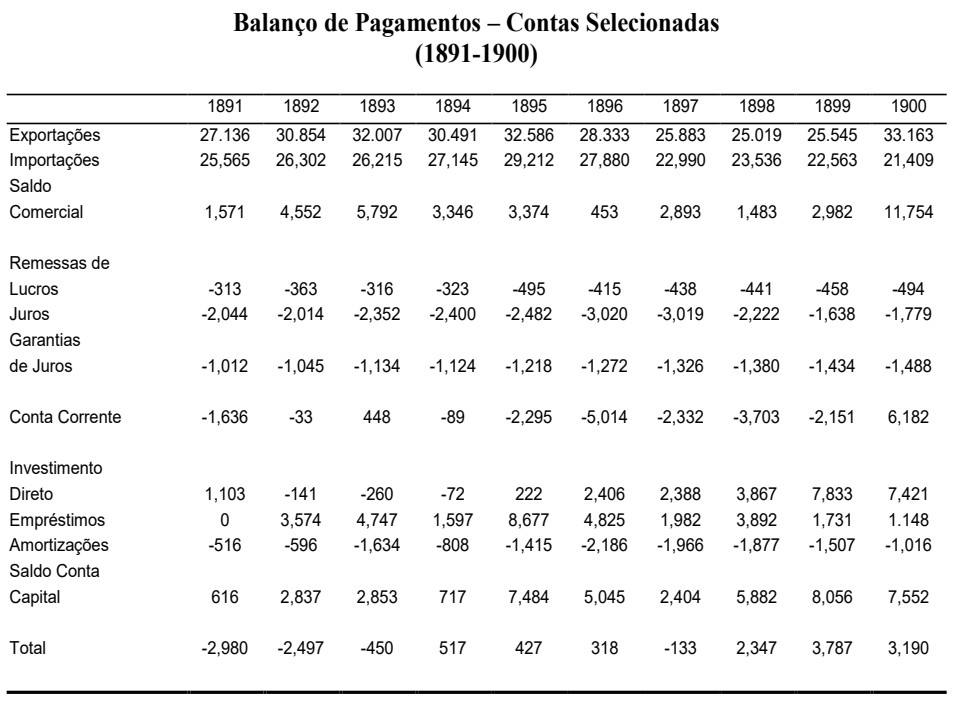
\includegraphics[width=0.5\textwidth]{Imagens Slides/i5a10.png}
    \caption{Balanço de Pagamentos – Contas Selecionadas (1891-1900)}
\end{figure}

\begin{figure}[H]
    \centering
    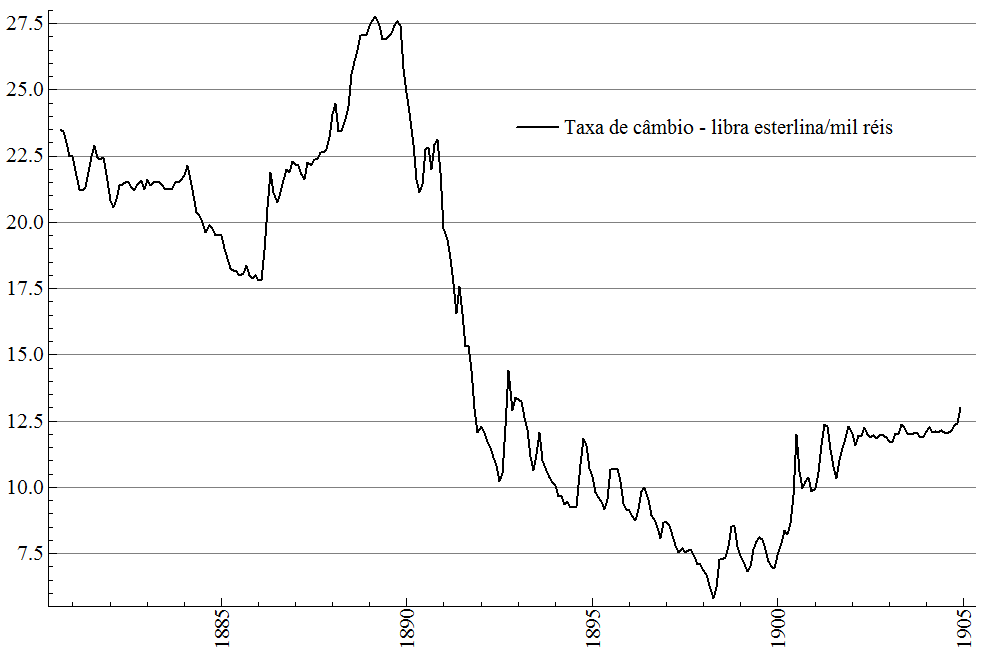
\includegraphics[width=0.5\textwidth]{Imagens Slides/i6a10.png}
    \caption{Taxa de Câmbio - libra esterlina/mil réis}
\end{figure}

\newpage

\section{\textbf{Aula 11 - Problemas econômicos e política econômica (1900-1930)}}

\subsection{\textbf{Objetivos e contexto}}
\begin{itemize}
    \item O que é importante?
    \begin{itemize}
        \item identificar e explicar os efeitos dos choques enfrentados pela economia brasileira bem como a reação de política econômica e desdobramentos;
    \end{itemize}
    \begin{itemize}
        \item Avaliar de forma crítica a lógica da política econômica.
    \end{itemize}
\textbf{Contexto}
    \item Flexibilização da hegemonia econômica inglesa
    \begin{itemize}
        \item  Inglaterra que liderou sozinha a 1ª Rev. Industrial enfrenta nesse período a concorrência de outros países (2ª Revolução Industrial)
    \end{itemize}
    \item Estado torna-se mais presente na economia
    \begin{itemize}
        \item redução gradual da liberdade comercial e financeira
    \end{itemize}
    \item Campo político brasileir
    \begin{itemize}
        \item  poderes regionais apoiam o poder federal em troca da consolidação do domínio regional. Agentes políticos são heterogêneos
    \end{itemize}
\end{itemize}
\subsection{\textbf{Introdução}}
\begin{itemize}
    \item Cenário internacional (choques exógenos) e a tendência ao desequilíbrio externo
    \begin{itemize}
        \item café com grande peso para o Brasil
    \end{itemize}
    \begin{itemize}
        \item  grandes variações de preços dadas flutuações da oferta de café (clima)
    \end{itemize}
    \begin{itemize}
        \item descontinuidade dos fluxos de capital para a periferia e variações das demandas dos países centrais são frequentes nos 1900-30
    \end{itemize}
    \item Quais podem ser as práticas de política econômica para enfrentar essa tendência?
\end{itemize}
\subsection{\textbf{Política econômica 1900-1913}}
\begin{itemize}
    \item Considerável crescimento econômico e relativa estabilidade de preços na média em 1900-13
    \item Melhora BP
    \begin{itemize}
        \item  grande crescimento das EX de borracha
    \end{itemize}
    \begin{itemize}
        \item boom de investimentos europeus na região (permanente até a véspera da I Guerra)
    \end{itemize}
    \item Permanece contração monetária
    \begin{itemize}
        \item inibe maior crescimento econômico
    \end{itemize}
    \begin{itemize}
        \item gera apreciação cambial que aliada a alta produção de café coloca dificuldades aos exportadores
    \end{itemize}
\item Criação da Caixa de conversão em 1906
\begin{itemize}
    \item  emissão de notas com plena conversibilidade em ouro
\end{itemize}
\begin{itemize}
    \item liga a oferta monetária doméstica ao comportamento do BP
\end{itemize}
\item Estimava-se para 1906 super-safra de café o que reduz receita com EX. Medidas possíveis:
\begin{itemize}
    \item PVC = mudar preço internacional do café através do controle da oferta mundial (facilitado pelo quase monopólio brasileiro e baixa elasticidade preço da demanda)
\end{itemize}
\begin{itemize}
    \item requer grande financiamento para estabelecer estoques não satisfeita dada a base bancária doméstica: buscar financiamento externo
\end{itemize}
\begin{itemize}
    \item solicitado apoio do governo para garantir empréstimos (governo nega ao Convênio de Taubaté)
\end{itemize}
\item 1907: dificuldade internacional
\begin{itemize}
    \item  não há rolagem do financiamento externo
\end{itemize}
\begin{itemize}
    \item governo busca garantir estabilidade macro, através da PVC
\end{itemize}
\begin{itemize}
    \item  governo federal entra de fato no processo de valorização do café, aumentando seu sucesso
\end{itemize}
\item Como a PVC melhora uma dificuldade no BP?
\item 1908: melhoria internacional
\begin{itemize}
    \item grande desempenho do BP: retornam fluxos de capital e aumento do pborracha,
resultando em expansão monetária
\end{itemize}
\begin{itemize}
    \item economia brasileira tem fase de grande crescimento econômico até 1913
\end{itemize}
\item 1908-1913
\begin{itemize}
    \item atividade interna determinada pela variação do BP (padrão ouro)
\end{itemize}
\begin{itemize}
    \item  fatores exógenos (fluxos de capital e preços das EX) são decisivos para determinar o nível da atividade
\end{itemize}
\item  Nesse contexto, quais são as possibilidades de ajustamento macroeconômico?
\begin{itemize}
    \item  supondo uma crise internacional, como o governo pode reagir?
\end{itemize}
\begin{itemize}
    \item quais as consequências esperadas na conjuntura?
\end{itemize}
\item 1900-11: grandes déficits orçamentários financiados por empréstimos externos
\item 1912: credores colocam grau de desconfiança, gerando dificuldades para novos empréstimos. Porque?
\begin{itemize}
    \item perspectiva baixa de crescimento das EX
\end{itemize}
\begin{itemize}
    \item pborracha em declínio
\end{itemize}
\begin{itemize}
    \item pcafé tem aumento (sucesso da PVC), mas reverte com ação americana
\end{itemize}
\item Deterioração externa brasileira em 1913 que na presença do padrão ouro
\begin{itemize}
    \item provoca forte arrocho monetário
\end{itemize}
\begin{itemize}
    \item economia brasileira já entra em recessão mesmo antes da I Guerra
\end{itemize}
\begin{itemize}
    \item  conjuntura passageira era a aposta brasileira e, assim, permanece no padrão ouro
\end{itemize}
\end{itemize}
\subsection{\textbf{Política econômica 1914-1918}}
\begin{itemize}
    \item I Guerra: afeta o comércio internacional e o fluxo
de pagamentos externos. Efeitos no Brasil?
\begin{itemize}
    \item receita tributária
\end{itemize}
\begin{itemize}
    \item economia cafeeira
\end{itemize}
\begin{itemize}
    \item  governo fecha a caixa de conversão
\end{itemize}
\item Medidas emergenciais
\begin{itemize}
    \item feriado bancário
\end{itemize}
\begin{itemize}
    \item moratória temporária de todas as dívidas
\end{itemize}
\begin{itemize}
    \item autoriza grande emissão inconversível para diminuir crises de liquidez e atender gastos do governo
\end{itemize}
\end{itemize}
\subsection{\textbf{Questão ANPEC 2001}}
\begin{itemize}
    \item Explique o que você entende por sistema
monetário do padrão-ouro e explicite as dificuldades dos países periféricos para
seguir suas regras. Que condições favoreceram o estabelecimento de uma Caixa de Conversão no Brasil no início do século? Que razões determinaram seu fechamento?
\end{itemize}

\begin{itemize}
    \item 1914: novo funding loan em outubro
    \begin{itemize}
        \item pagar juros até 1917 e suspensão das amortizações até 1927
    \end{itemize}
    \begin{itemize}
        \item aliviar pressão sobre o BP
    \end{itemize}
    \begin{itemize}
        \item  estagnação das importações
    \end{itemize}
    \begin{itemize}
        \item desequilíbrio fiscal do governo tende a ficar permanente dada a dependência da receita em relação à tarifa sobre as IM
    \end{itemize}
    \begin{itemize}
        \item  queda de 8,7\% da produção industrial
    \end{itemize}
\item 1915 (Guerra permanece, promover ajustes)
\item  Equacionar o setor público
\begin{itemize}
    \item reduzir despesas
\end{itemize}
\begin{itemize}
    \item ampliar base de produtos para tributação de consumo
\end{itemize}
\begin{itemize}
    \item reduz déficit em termos reais
\end{itemize}
\item  Reverter aperto monetário
\begin{itemize}
    \item nova autorização para emissão de notas do tesouro e títulos federais de longo prazo para cobrir despesas e fornecer crédito
\end{itemize}
\item 1916: piora da balança comercial
\begin{itemize}
    \item economia de guerra (restrição das importações de café e da navegação)
\end{itemize}
\begin{itemize}
    \item agravada pela previsão de grande safra de café
\end{itemize}
\item  1917: crescem estoques de café
\begin{itemize}
    \item novas emissões inconversíveis para comprar a safra
\end{itemize}
\begin{itemize}
    \item  ↑ preços alimentos; ↓ salário real, geram greves e manifestações
\end{itemize}
\item 1918
\item  1ª metade: mantido o cenário do ano anterior
\begin{itemize}
    \item preocupação com a fragilidade externa e com a economia cafeeira
\end{itemize}
\item  2ª metade: pcafé
\begin{itemize}
    \item finalização da I Guerra
\end{itemize}
\begin{itemize}
    \item ocorrência de geadas (quebram colheitas, trazendo depressão da atividade doméstica)
\end{itemize}
\begin{itemize}
    \item Brasil nesse período não apresenta excesso de oferta de café e há equilíbrio externo
\end{itemize}
\end{itemize}
\subsection{\textbf{Política econômica 1919-1922}}
\begin{itemize}
    \item 1919: boom internacional
    \begin{itemize}
        \item ↑ p commodities; ↓oferta de café e diversificação da pauta exportadora conquistada no período de Guerra: ↑ explosivo das EX
    \end{itemize}
\begin{itemize}
    \item recuperação da atividade doméstica
\end{itemize}
\begin{itemize}
    \item apreciação do mil-réis (abandono das paridades na Europa)
\end{itemize}

\begin{itemize}
    \item  há demanda por importações, mas há desestruturação internacional
\end{itemize}
\begin{itemize}
    \item  Brasil fecha o ano com grande superávit comercial
\end{itemize}
\item 1920: pressão inflacionária combatida com política monetária restritiva, gerando recessão nos EUA e UK
\begin{itemize}
    \item ↓p dos primários
\end{itemize}
\item Brasil
\begin{itemize}
    \item ↓EX
\end{itemize}
\begin{itemize}
    \item  ↑IM: pressão importadora e apreciação cambial do ano anterior
\end{itemize}
\begin{itemize}
    \item reversão da balança comercial
\end{itemize}
\item 1920: desvalorização cambial
\begin{itemize}
    \item efeitos: déficit orçamentário (despesas em moeda estrangeira e arrecadação ligada a alfândega); salários reais (impacto inflacionário – alimentos) e setor cafeeiro
\end{itemize}
\begin{itemize}
    \item  medida: cria-se o emprestador “automático” de última instância (notas do tesouro e carteira de Redesconto do BB)
\end{itemize}
\item 1921: dificuldade de financiar o crescente
desequilíbrio fiscal
\begin{itemize}
    \item recorre ao crédito externo para financiar PVC (preço favorável e expectativa de colheita menor)
\end{itemize}
\begin{itemize}
    \item  sucesso da PVC, controlando queda do pcafé
\end{itemize}
\item 1922: agrava a situação fiscal
\begin{itemize}
    \item financia via letras de curto prazo e redesconto de títulos federais ( ↑ base monetária, gerando pressão inflacionária)
\end{itemize}
\item Fim de 1922: efeitos da PVC
\begin{itemize}
    \item  ↑ pcafé
\end{itemize}
\begin{itemize}
    \item melhora das exportações e do déficit comercial
\end{itemize}
\begin{itemize}
    \item  alto nível da construção civil, pois há obras públicas e expansão de crédito
\end{itemize}
\item BB dotado do monopólio da emissão
\item Acelera depreciação do mil-réis (emissão do BB frente crise de liquidez)
\begin{itemize}
    \item governo cogita empréstimo externo para evitar crises cambial e fiscal
\end{itemize}
\begin{itemize}
    \item há efeito inflacionário e queda do salário real
\end{itemize}
\item Missão inglesa (1924) fornece as bases (condicionantes) do empréstimo para o governo
\begin{itemize}
    \item choque monetário
\end{itemize}
\begin{itemize}
    \item esforço fiscal para equilibrar orçamento
\end{itemize}
\begin{itemize}
    \item posição externa frágil (↑EX “anulada” pelo ↑IM, pois há recuperação doméstica)
\end{itemize}
\end{itemize}
\subsection{\textbf{Política econômica 1925-1926}}
\begin{itemize}
    \item Política contracionista: gera conjuntura recessiva
    \begin{itemize}
        \item ↓ inflação
    \end{itemize}
    \begin{itemize}
        \item apreciação cambial
    \end{itemize}
    \begin{itemize}
        \item estagnação da produção industrial
    \end{itemize}
    \item  Retorno ao padrão-ouro
    \begin{itemize}
        \item  PVC melhora pcafé
    \end{itemize}
    \begin{itemize}
        \item grande investimento estrangeiro
    \end{itemize}
    \begin{itemize}
        \item superávit no BP possibilita emissões ao longo do tempo (1927-28)
    \end{itemize}
\end{itemize}
\subsection{\textbf{Política econômica 1927-1928}}
\begin{itemize}
    \item Há expansão econômica com estabilidade de preços
    \begin{itemize}
        \item dependente das condições internacionais favoráveis
    \end{itemize}
    \begin{itemize}
        \item há estabilidade cambial
    \end{itemize}
    \begin{itemize}
        \item capacidade ociosa no setor industrial
    \end{itemize}
    \item Piora da situação externa (2ª metade de 1928)
    \begin{itemize}
        \item crescimento das IM compromete saldo comercial (forte redução do saldo)
    \end{itemize}
    \begin{itemize}
        \item reduz fluxo de empréstimos estrangeiros
    \end{itemize}
    \begin{itemize}
        \item  ↓ emissões da caixa de estabilização
    \end{itemize}
\end{itemize}
\subsection{\textbf{Política econômica 1929-1930}}
\begin{itemize}
    \item 929 é ano de uma super-safra de café: Brasil já apresenta tendência recessiva antes mesmo da crise financeira
    \begin{itemize}
        \item  deflação econômica
    \end{itemize}
    \begin{itemize}
        \item  crise de 29 impede qualquer financiamento externo, assim é inviável promover a PVC
    \end{itemize}
    \item 1930 apresenta queda nos preços do café o que agrava situação do BP, mas o governo acredita em crise passageira
\end{itemize}
\subsection{\textbf{Disussão importante}}
\begin{itemize}
    \item Práticas de política econômica, na República Velha, foram voltadas para os interesses do café? Considerar os aspectos abaixo
    \begin{itemize}
        \item planos de valorização do café
    \end{itemize}
    \begin{itemize}
        \item  tendência cambial
    \end{itemize}
    \begin{itemize}
        \item  padrão-ouro como regime monetário
    \end{itemize}
\end{itemize}
\subsection{\textbf{Conclusão: O que aprendemos?}}
\begin{itemize}
    \item Aplicar conteúdo da macroeconomia para explicar e avaliar a conjuntura econômica brasileira
    \begin{itemize}
        \item avaliar e explicar os efeitos da adoção e abandono do padrão-ouro
    \end{itemize}
    \begin{itemize}
        \item  explicar os efeitos da prática da PVC
    \end{itemize}
    \item Identificar e explicar as consequências da IGM e quais foram as reações de política econômica
    \item Identificar e explicar as consequências de uma depreciação cambial nos anos 1920
    \begin{itemize}
        \item  entender a importância da estrutura de endividamento
    \end{itemize}
    \begin{itemize}
        \item notar a transmissão dos efeitos (inflação, ciclo do café, produção nacional)
    \end{itemize}
    \begin{itemize}
        \item explicar a política econômica para combater os efeitos
    \end{itemize}
    \item Avaliar as opções de política econômica e as consequências observadas
    \begin{itemize}
        \item  explicar o papel e os efeitos de um ajuste fiscal
    \end{itemize}
    \begin{itemize}
        \item avaliar o papel das expectativas
    \end{itemize}
\end{itemize}
\newpage

\section{\textbf{Aula 12 - Política econômica e problemas econômicos no período 1930-1945}}

\subsection{\textbf{Introdução}}
Três subperíodos definem o contexto de 1930-1945:
    \begin{itemize}
        \item Governo vive crise e recuperação de 1930 a 1934
        \item Há certa liberalização da política econômica no período de 1934 a 1937
        \item Até 1945 a economia brasileira enfrenta uma recessão americana e os anos da II Guerra
    \end{itemize}

\subsection{\textbf{1930 - 1934}}
\begin{itemize}
    \item Efeitos da crise e enfrentamento brasileiro (retomada da segunda parte da última discussão)
    \begin{itemize}
        \item Furtado versus Pelaez;
        \item Qualificações para esse debate (Silber, Cardoso e Haddad);
        \item Crescimento do déficit fiscal;
        \item Política econômica favoreceu a indústria;
        \item ↑ saldo comercial (desvalorização e controle cambial).
    \end{itemize}
\end{itemize}

\begin{itemize}
    \item Política Monetária
    \begin{itemize}
        \item abandono do padrão-ouro em meados de 1930;
        \item crescimento forte da base monetária a partir de 1932.
    \end{itemize}
    \item Instituições
    \begin{itemize}
        \item Bancos resistem a crise – regulação forte é histórica no Brasil;
Governo reforça a operação de descontos títulos via carteira do BB, financiando Tesouro e PVC
    \end{itemize}
    \item Inflação
    \begin{itemize}
        \item queda de preços no período 1930/31;
        \item certa estabilidade em 1932/33.
    \end{itemize}
\end{itemize}

{\textbf{Setor industrial}}
\begin{itemize}
    \item Indústria
    \begin{itemize}
        \item  $PIB_{Ind}$ cresce de 1932 até 1939;
        \item descola do desempenho do café;
        \item comportamento difere do contexto da Primeira República;
        \item sugere, de fato, o início da fase de industrialização do Brasil (Baer, W.);
        \item evidências (Haddad, C.).
    \end{itemize}
\end{itemize}

\subsection{{\textbf{Lógica da política econômica}}}
\begin{itemize}
    \item Qual foi a lógica a partir de 1930? Como era antes?
    \begin{itemize}
        \item agora, aspectos internos parecem dominar as preocupações e motivam mais a política econômica;
        \item setor industrial ganha atenção do governo;
        \item contexto internacional é outro, mais intervencionista;
        \item Lógica do padrão-ouro questionada;
        \item PVC mais sob a motivação de estimular o produto; 
        \item equilíbrio externo viria mais com controles do governo dado o cenário de escassez de divisas;
        \item Exemplo de controle: mercado de câmbio.
    \end{itemize}
\end{itemize}

\subsection{{\textbf{Setor externo (BP), 1930 1945}}}
\begin{itemize}
    \item No geral, a balança comercial foi superavitária
    \item A balança de serviços, por outro lado, foi deficitária, gerando transações correntes negativas
    \item A conta de capitais mostrou grande restrição em grande parte do tempo
    \item Em suma, um período de escassez/instabilidade de divisas com pequena sobra de reservas internacionais
\end{itemize}

\subsection{\textbf{Controle cambial, 1931 - 1938}}
\begin{itemize}
    \item Contexto
    \begin{itemize}
        \item depressão reduz receita cambial brasileira;
        \item há pagamentos da dívida externa, remessas de lucros e importações;
        \item há desequilíbrio no mercado de câmbio;
        \item tentar limitar a demanda (suspender pagamentos da dívida), mas dificuldades persistem;
        \item implementar o controle cambial.
    \end{itemize}
    \item  O que significa? Como funcionou
    \begin{itemize}
        \item os cambiais obtidos com as EX tem de ser vendidos ao BB;
        \item BB vende a uma taxa oficial, seguindo prioridades definidas pelo Governo;
        \item 1) compras do Governo e dívida externa;  2) IM essenciais e 3) Outros, inclusive para remessa de lucros.
    \end{itemize}
\end{itemize}
\begin{itemize}
    \item Objetivo: equilibrar BP. Efeitos?
    \begin{itemize}
        \item dificulta IM menos essenciais;
        \item favorece indústria, já beneficiada pela depreciação;
        \item a dificuldade cambial melhora somente em 1934;
        \item surge um mercado cambial paralelo (taxa maior que oficial);
        \item o controle cambial é flexibilizado ao longo do tempo a medida em que aumenta a oferta de cambiais;
        \item em 1935 cambiais não obtidos com as EX são autorizados a operar no mercado livre (tentar reduzir mercado paralelo);
    \end{itemize}
\end{itemize}

\subsection{\textbf{1934 - 1937}}
\begin{itemize}
    \item Efeitos na prática do controle cambial
    \begin{itemize}
        \item mercado de câmbio alvo de pressões
(americanas);
\item câmbio para as EX variou, mas foi quase constante para as IM;
\item há acúmulo de reservas cambiais pelo BB (dados esse controle e a melhora do café);
\item isso permite liberar remessa de lucros. O objetivo é atrair capitais (frustrado dada a recessão americana em 1937/38).

    \end{itemize}
\end{itemize}

\subsection{Dívida externa e investimento estrangeiro (1930/45)}
\begin{itemize}
    \item Composição da dívida e fluxo de investimentos
    \begin{itemize}
        \item estoque maior em libras, mas o peso do dólar é maior desde a década de 1920;
        \item peso dos credores americanos é grande;
        \item ↓ IDE (dificuldade internacional e crise cambial brasileira).
    \end{itemize}
    \item Fluxos variam de acordo com:
    \begin{itemize}
        \item Intervenções do governo brasileiro;
        \item Contexto global;
        \item Diplomacia.
    \end{itemize}
\end{itemize}

\subsection{Investimento estrangeiro e diplomacia (1930/45)}
\begin{itemize}
    \item As relações comerciais pós Crise de 29
declinaram
\begin{itemize}
    \item Há escassez de liquidez, por isso, o investimento direto estrangeiro importa;
\item Estado regula onde são permitidos os investimentos estrangeiros
\item Setores estratégicos com restrição (por exemplo, mineração e recursos hídricos)
\item promover nacionalização de indústrias “essenciais”;
\item ↓ IDE (exceto o americano que sobe após 36);
\item a regulação pode ter interferido, mas a conjuntura internacional parece ser a explicação principal para a queda do IDE.
\end{itemize}
\end{itemize}

\subsection{Atividade econômica (1930/45)}
\begin{itemize}
    \item O contexto inicial foi, sobretudo, recessivo
    \begin{itemize}
        \item Evidências: 14 trimestres consecutivos em recessão, incluindo o pré Crise de 29 (Vieira e Valls, 2013)
        \item Recessão termina em 1932 (3), recuperação, relativamente, rápida
    \end{itemize}
    \item O período pré Estado Novo, 1934/37 
    \begin{itemize}
        \item Mostra crescimento médio forte, de 6,5\% aa;
        \item Agricultura 2\% e Indústria 11\% aa;
    \end{itemize}
\end{itemize}
\subsection{Mudança política importante}
\begin{itemize}
    \item Golpe militar, continuidade de Getúlio Vargas;
    \begin{itemize}
        \item reverte descentralização republicana (e enfraquece oligarquias cafeeiras);
    \end{itemize}
    \begin{itemize}
        \item Suspensão do legislativo, dos partidos e censura a imprensa;
    \end{itemize}
    \begin{itemize}
        \item criação do salário mínimo (1940), CLT (1943) e controle dos sindicatos;
    \end{itemize}
    \begin{itemize}
        \item governo interfere na regulação econômica, passando de normativo para provedor de bens e serviços, induzindo a industrialização (ISI) – nacionalismo econômico.
    \end{itemize}
\end{itemize}

\subsection{Atividade econômica (1930/45)}
\begin{itemize}
    \item 1937/45
    \begin{itemize}
        \item economia brasileira mostra desempenho fraco;
    \end{itemize}
    \begin{itemize}
        \item setor agrícola estagnado e setor industrial reduz sua taxa de crescimento;
    \end{itemize}
    \begin{itemize}
        \item Brasil somente anota crescimento após 1942;
    \end{itemize}
    \begin{itemize}
        \item O término da recessão ocorre antes do final da Guerra, mas o Brasil observa um surto inflacionário
    \end{itemize}
\end{itemize}

\subsection{Retorno a liberdade cambial, 1939-1946}
\begin{itemize}
    \item Há melhoria do mercado cambial em meados de 1939 e o governo cria três taxas: livre, oficial e livre especial
    \begin{itemize}
        \item a taxa livre é determinada pelo mercado, abastecido pelos cambiais das EX (30\% destinada ao BB à taxa
oficial);
\item a oficial, administrada pelo BB era para prover cambiais para o Governo;
\item a livre especial é para turismo e viagem.
    \end{itemize}
    \item A II Guerra, exceto no início, traz grandes saldos comerciais para o Brasil
    \begin{itemize}
        \item a Guerra restringiu as IM, na prática um controle cambial
    \end{itemize}
\end{itemize}

\subsection{1937-1945}
\begin{itemize}
    \item Episódio de surto inflacionário (1939-1945)
    \begin{itemize}
        \item políticas fiscal, monetária e creditícias são expansionistas;
        \item financiamento do déficit fiscal via emissão monetária a partir de 1942;
        \item aumento de empréstimos do BB e dos bancos comerciais
        \item  ↑ Saldo comercial: há restrição às IM e competição entre consumo doméstico e exportação (carne);
        \item  esforços brasileiros no combate a esse surto são tímidos.
    \end{itemize}
    \item Contexto da II Guerra Mundial
    \begin{itemize}
        \item ↑ dependência com os EUA (tanto para EX quanto para IM);
        \item 60\% das $EX_{BRA}$ seguem para os EUA;
        \item desenvolver Brasil significa mercado para $EX_{EUA}$;
    \end{itemize}
\end{itemize}

\subsection{Indústria e II Guerra Mundial}
\begin{itemize}
    \item Similar ao contexto da I Guerra Mundial 
    \item Alguns setores aproveitam e ampliam EX. Destaque para a têxtil que aproveita a Guerra
    \begin{itemize}
        \item mas perde espaço rápido com o fim da Guerra. 
    \end{itemize}
    \item Produção industrial mais diversificada
    \begin{itemize}
        \item setor de bens de capital cresce de forma limitada;
        \item bens intermediários são destaque com metalurgia e química (expansão da Ind. Siderúrgica).
    \end{itemize}
    \item  Indústria passa a ser o setor de ponta

 
\end{itemize}

\subsection{Resultados finais do período 1930-1945}
\begin{itemize}
    \item Pressão inflacionária sugere excessos da política econômica
    \item Brasil passou por um período longo de restrições externas
    \item Aproximação com EU
    \item  Instalação do setor de bens intermediários (diversificação industrial)
\end{itemize}

\subsection{Conclusão: o que aprendemos e porque?}
\begin{itemize}
    \item Aplicar conteúdo da macroeconomia para explicar e avaliar a conjuntura econômica brasileira
    \begin{itemize}
        \item avaliar e explicar os efeitos da adoção do controle cambial
        \item explicar os efeitos da prática da PVC na década de 1930
    \end{itemize}
    \item Identificar e explicar as consequências da IIGM e quais foram as reações de política econômica
\item  Identificar e explicar as consequências do surto inflacionário nos anos 1940
\begin{itemize}
    \item explicar a política econômica para combater os efeitos 
\end{itemize}
\item Avaliar as opções de política econômica e as consequências observadas
\begin{itemize}
    \item explicar o papel e os efeitos da política monetária
    \item avaliar o papel das expectativas
\end{itemize}
\end{itemize}

\section{\textbf{Aula 13 - Setor externo e política cambial no período 1946 - 1954}}

\subsection{Introdução}
\begin{itemize}
    \item Permanece o cenário de escassez de divisas nos dois governos
\end{itemize}
\begin{itemize}
    \begin{itemize}
        \item Resultados da balança comercial são oscilantes;
    \end{itemize}
\end{itemize}
\begin{itemize}
    \begin{itemize}
        \item Ainda há dependência do fluxo de capitais norte americano.
    \end{itemize}
\end{itemize}
\begin{itemize}
    \item Diante da dificuldade do setor externo os governos recorrem à prática do controle de câmbio
\end{itemize}

\subsection{Governo Dutra}
\begin{itemize}
    \item A avaliação inicial do governo mostrou que o setor externo estava equilibrado 
    \begin{itemize}
        \item  O Brasil tinha acumulado reservas durante a II Guerra;
        \item O sistema monetário global seria reorganizado no pós Guerra;
        \item Por isso, a atenção do governo se voltou para tentar resolver o problema inflacionário
    \end{itemize}
    \item Mas essa avaliação sobre o setor externo se mostrou equivocada
\end{itemize}

\subsection{Política cambial no governo Dutra}
\begin{itemize}
    \item Movimento de capitais 
\end{itemize}
Dutra contava com o fluxo de capitais estrangeiros através do apoio americano e da melhoria internacional. 
\begin{itemize}
    \begin{itemize}
        \item Para atrair capital, inicialmente, executa política cambial liberal;
        \item Mas os EUA não estão preocupados com o Brasil e sim com a Europa;
        \item Assim, o Brasil dependeria de fluxos privados;
        \item Mas há fortes estrangulamentos de energia e de transporte.
    \end{itemize}
\end{itemize}
Por isso, o financiamento externo é precário.

\begin{itemize}
    \item Agravante: disponibilidade de divisas era uma “ilusão”
    \begin{itemize}
        \item Brasil tinha superávit com moedas inconversíveis! O que deixa enganosa o superávit e equilíbrio até 1948;
        \item Brasil necessitava acumular dólar e não moedas fracas;
        \item Desvalorizar o câmbio foi descartado dados os objetivos do Governo (traria inflação e não frearia importações de insumos industriais, dada sua inelasticidade).


    \end{itemize}\end{itemize}
    O regime de câmbio é fixo. A escolha foi voltar com o controle cambial

 1947 – início dos controles cambiais e de importações (similar ao da década de 30). Havia licenças prévias para importar de acordo com as prioridades do Governo.
     \begin{itemize}
         \item objetivo era reduzir o déficit na área que gerava moedas conversíveis;
         \item há redução desse déficit ao longo do tempo
     \end{itemize}
 Câmbio fixo, diante do contexto inflacionário e de controle cambial:
     exportações brasileiras perderam competitividade, dado o movimento global de desvalorização;
     produtos brasileiros que se beneficiaram no período da Guerra perdem espaço;
     Inflação brasileira supera mundial, ou seja, câmbio real valorizado;

\subsection{Fim do governo Dutra}
\begin{itemize}
    \item Proximidade das eleições gera forte aumento de gastos (União e estados);
\end{itemize}
\begin{itemize}
    \item Há política de crédito ativa para o setor industrial
\end{itemize}
 \begin{itemize}
     \item Na prática, fim da ilusão liberal e das práticas econômicas ortodoxas
 \end{itemize}
     \begin{itemize}
         \item Há retomada do crescimento, da inflação e do déficit orçamentário;


     \end{itemize}


\textbf{ Síntese}: a condução liberal foi substituída por medidas que incentivaram o setor industrial, dada as restrições externas e pressões internas por crédito
\subsection{Vargas}
1º Fase
\begin{itemize}
    \item Reequilibrar as finanças públicas e fazer política monetária restritiva para controlar o crescimento da inflação.

2º Fase
\item Realizar os empreendimentos (infraestrutura para projetos industriais), que dependem:
\begin{itemize}
    \item do sucesso da 1ª fase;
    \item da entrada de capitais estrangeiros (CMBEU, 1951, Comissão Mista Brasil-EUA, que explorava o ponto de Truman (1949) - auxiliar países do Terceiro Mundo via Banco Mundial e Eximbank (Banco de exportação e importação)
\end{itemize}
    \item Há elevação das importações (destaque bens de capital):
    \begin{itemize}
        \item expansão de crédito
        \item liberação de importações com afrouxamento das licenças;
        \item cruzeiro sobrevalorizado;
        \item setor privado aumenta a taxa de investimento dado o contexto que permite e incentiva a elevação de importados, ampliando participação em relação a
parcela pública.
    \end{itemize}
    \item Em 1952 reduzem as receitas de exportação 
    \begin{itemize}
        \item cruzeiro sobrevalorizado e pressão inflacionária interna,
        \item crise na indústria têxtil mundial reduz exportações de algodão
        \item expectativa de desvalorização faz exportadores reterem estoques
        \item exceto o café
    \end{itemize}
    \item Resultados
    \begin{itemize}
        \item  déficit na balança comercial, esgotamento das reservas internacionais
        \item crise cambial (1952/53)
        \item fluxo de capitais não amenizou essa crise, comprometendo o projeto Campos Sales-Rodrigues Alves.
    \end{itemize}
    \item  Relações internacionais 
    \begin{itemize}
        \item mudança política nos EUA (1953), Eisenhower, Republicano, interrompe 20 anos de governos democratas (tira o olhar sobre os países latino americanos);
        \item objetivo, agora, é barrar o comunismo na Europa e reduzir gastos e interferências globais fora desse foco;
        \item Vargas rompeu com os organismos financeiros americanos;
        \item por isso, Banco Mundial rompe o envio de recursos para o Brasil.
    \end{itemize}
\end{itemize}

\subsection{Lei do Mercado Livre}
\begin{itemize}
    \item Diante da escassez de divisas, a SUMOC institui a Lei no 1.807, janeiro de 1953, Lei do Mercado Livre:
    \begin{itemize}
        \item mercado livre de câmbio para o capital estrangeiro no Brasil e para as importações não essenciais;
    \end{itemize}
    \begin{itemize}
        \item instituiu as taxas múltiplas de câmbio: uma paridade declarada (mais valorizada) e uma determinada pelo mercado (mais desvalorizada);
    \end{itemize}
    \begin{itemize}
        \item as diferentes taxas buscavam, ao mesmo tempo, incentivar exportações (gravosos) e permitir vantagens às importações essenciais;
        \item poderia pressionar a inflação;
        \item mas políticas monetária e creditícia seriam contracionistas e evitariam essa eventual pressão.
    \end{itemize}

\end{itemize}
\begin{itemize}
    \item Resultados
    \item havia expectativa de mais desvalorização, o que gerou atraso de exportações e antecipações de importações;
    \begin{itemize}
        \item piora das EX (gravosos não reagiram e café mostrou perdas);
    \end{itemize} 
    \begin{itemize}
        \item capitais estrangeiros também não reagiram, IDE até piorou.
    \end{itemize}
\end{itemize}
\subsection{Instrução da SUMOC e a situação cambial}
\begin{itemize}
    \item Diante da piora cambial, o governo institui a Instrução 70 da SUMOC, outubro de 53
    \begin{itemize}
        \item Objetivos: incentivar as EX, encarecer as IM com mecanismos de mercado (os leilões), manter seleção de IM e ampliar arrecadação fiscal
    \end{itemize}
    \item  BB retoma o monopólio cambial;
    \item Cria os leilões de câmbio:
    \begin{itemize}
        \item  (1) Taxa oficial, sem sobretaxa, para trigo, papel imprensa;
        \item (2) Taxa oficial, com sobretaxa fixa, para as importações do governo;
        \item (3) Taxa oficial, com sobretaxa variável (a depender do lance feito em leilão), para as demais importações categorizadas em ordem decrescente de essencialidade
    \end{itemize}
\end{itemize}

\subsection{Segundo Vargas}
\begin{itemize}
    \item  Em 1954, a lógica contracionista de Aranha não foi alterada, mas as condições forçaram grande crescimento creditício
    \begin{itemize}
        \item demanda dos estados, política do café e aumento do salário mínimo em 100\% dado por Vargas;
    \end{itemize}
    \begin{itemize}
        \item a proposta foi de João Goulart com forte oposição da FIESP, militares, Aranha, (que sugeriam 30\%)
    \end{itemize}
    \begin{itemize}
        \item situação se agrava quando, contrariando expectativas, o café tem exportações reduzidas no início do ano (EUA promovem campanha para menor consumo )

    \end{itemize}
\end{itemize}


Assim, a política de Aranha foi fortemente prejudicada pelas dificuldades do café, repasses inflacionários a partir das desvalorizações cambiais, aumento do salário mínimo e expansão de crédito que inviabilizaram a austeridade.


\section{\textbf{Aula 14 - O governo de Café Filho (1954/1955)}}

\subsection{Café Filho, 1954 - 1955}
Texto: EBC (Cap. 1, trecho sobre Café Filho) 
\begin{itemize}
    \item O que é importante?
    \begin{itemize}
        \item Notar que a prática fortemente ortodoxa implementada por Gudin foi, basicamente, anulada por Whitaker (foram 3 ministros em um ano!)
    \end{itemize}
    \item Conjuntura externa e a gestão de Gudin   
    \begin{itemize}
        \item colapso cambial em meados de 1954 ( diminuição do preço do café);
        \item  agentes econômicos internacionais, mostram-se receptivos à Gudin.
    \end{itemize}
\end{itemize}

\subsection{A gestão de Gudin}
\begin{itemize}
    \item Governo Eisenhower ainda dificulta as negociações e a disposição dos agentes oficiais.
    \begin{itemize}
        \item  setor privado deve enviar capitais, não são recursos públicos que devem financiar a América Latina.
    \end{itemize}
    \item Nesse sentido, a melhoria do BP dependeria da política econômica interna e Gudin defendia a livre entrada de capital estrangeiro.
\end{itemize}

\subsection{Café Filho}
\begin{itemize}
    \item Estabilização de Gudin
    \begin{itemize}
        \item elevação da taxa de juros;
        \item aumento do compulsório sobre os depósitos à vista e a prazo, com recolhimento a SUMOC e não mais ao BB (item importante da Instrução 108), evitando possível fuga via expansão de crédito;
        \item estabelecidos limites de operações para carteiras do BB, identificadas como o foco da expansão monetária ao ceder recursos para o Tesouro;
        \item pretendia atrelar o crescimento dos gastos ao crescimento da receita, mas não viabilizou politicamente. A opção do executivo foi cortar investimentos públicos em vez de gastos correntes com consumo!
    \end{itemize}
    \item Efeitos do plano ortodoxo:
    \begin{itemize}
        \item grave crise de liquidez em 55, gerando falências, corrida bancária, liquidação de bancos e queda do investimento privado e público (FBCF) e das importações de bens de
capital;
\item não houve queda do produto industrial;
\item em termos históricos, isso é uma desaceleração econômica (período não datado como uma recessão);
\item período do Ministro Gudin foi curto.
    \end{itemize}
\end{itemize}

\subsection{A reforma cambial de 1955}
\begin{itemize}
    \item Instrução 113, autoriza entrada de bens de capital “sem cobertura cambial”
    \begin{itemize}
        \item Permite importar diretamente bens de capital na forma de IDE (sem licenças);
        \item Estimulou ingressos de capital estrangeiro
    \end{itemize}
    \item Tal reforma seria uma crítica ao formato de industrialização que vinha sendo praticada (crises no BP como consequência da PSI).
    \begin{itemize}
        \item Permitiria industrializar sem pressionar o BP (aliviando IM)
        \item Não pressionaria inflação (pois não afeta a base monetária)
    \end{itemize}
\end{itemize}

\subsection{Café Filho}
\begin{itemize}
    \item A gestão de José Maria Whitacker 
    \begin{itemize}
        \item banqueiro paulista nomeado para tentar acalmar a plutocracia paulista;
        \item crítico das taxas múltiplas e defensor do setor agrícola;
        \item reverter política econômica para reverter a crise de liquidez deixada por Gudin (inflação não seria preocupação central);
        \item pede liberação de crédito via BB (para setores produtivos);
        \item revoga medidas anteriores, como as taxas de compulsório e de redesconto anteriores.
    \end{itemize}
\end{itemize}


Síntese: Um ano de transição com três ministros, o segundo tomando medidas que praticamente anularam as do primeiro.

 
\end{document}




